% BU ECE template for MS thesis and PhD dissertation.
%
%==========================================================================%
% MAIN PREAMBLE 
%==========================================================================%
\documentclass[12pt,letterpaper]{report}          % Single-sided printing for the library
%\documentclass[12pt,twoside]{report} % Double-sided printing
\usepackage[intlimits]{amsmath}
\usepackage{amsfonts,amssymb}
\DeclareSymbolFontAlphabet{\mathbb}{AMSb}
% Handles references
\usepackage[backend=biber, bibencoding=utf8, maxcitenames=2, uniquelist=false, style=authoryear-comp, natbib=true]{biblatex}  
\usepackage{float}
\usepackage[bf]{caption}       
\setcaptionmargin{0.5in}
\usepackage{fancyhdr}
%\usepackage{fancyheadings}
\usepackage{fancybox}
\usepackage{ifthen}
\usepackage{bu_ece_thesis}
\usepackage{url}
\usepackage{lscape,afterpage}
\usepackage{xspace}
\usepackage{epstopdf} 
\usepackage{placeins}
\usepackage{multirow}
% Handle units
\usepackage{siunitx}
% Handle lists
\usepackage{enumitem}
% Handle colors
\usepackage{xcolor}
% Handle tables
\usepackage{tabularx, caption}
% Handle figures
\usepackage{graphicx, subcaption}
% Handle paragraph formatting
\edef\restoreparindent{\parindent=\the\parindent\relax}
\usepackage{parskip}
\restoreparindent
% Add line numbers
\usepackage{lineno}
% Handle units
\usepackage{siunitx}
% Provide subsubsubsections
\usepackage{titlesec}
% To accommodate UTF encoding
\usepackage[utf8]{inputenc} 
% Handle math
\usepackage{amsmath}
\addbibresource{thesis.bib}

%==========================================================================%
%%% graphicx and pdf creation
\usepackage{graphicx}
\usepackage{appendix}
%\usepackage{psfrag}
%\DeclareGraphicsExtensions{.eps}   % extension for included graphics
%\usepackage{thumbpdf}              % thumbnails for ps2pdf
\usepackage[ps2pdf,                % hyper-references for ps2pdf
bookmarks=true,%                   % generate bookmarks ...
bookmarksnumbered=true,%           % ... with numbers
hypertexnames=false,%              % needed for correct links to figures !!!
breaklinks=true,%                  % breaks lines, but links are very small
linkbordercolor={0 0 1},%          % blue frames around links
pdfborder={0 0 112.0}]{hyperref}%  % border-width of frames 
%==========================================================================%
% customized commands can be placed here
%\newcommand{\figref}[1]{Figure~\ref{#1}}
%\newcommand{\chapref}[1]{Chapter~\ref{#1}}
%\newcommand{\latex}{\LaTeX\xspace}
%==========================================================================%

%==========================================================================%
% BEGIN
%==========================================================================%
\begin{document}

% The preliminary pages
% This file contains all the necessary setup and commands to create
% the preliminary pages according to the buthesis.sty option.

\title{Understanding the relationship between urban areas and the boundary layer using remote sensing methods}

\author{Gabriel Angel Rios}

\department{Department of Mechanical Engineering}

% Degree year is the year the diploma is expected, and defense year is
% the year the dissertation is written up and defended. Often, these
% will be the same, except for January graduation, when your defense
% will be in the fall of year X, and your graduation will be in
% January of year X+1
\degreeyear{2022}

% For each reader, specify appropriate label {First, Second, Third},
% then name, and title. IMPORTANT: The title should be:
%   "Professor of Electrical and Computer Engineering",
% or similar, but it MUST NOT be:
%   Professor, Department of Electrical and Computer Engineering"
% or you will be asked to reprint and get new signatures.
% Warning: If you have more than five readers you are out of luck,
% because it will overflow to a new page. You may try to put part of
% the title in with the name.
\reader{First}{Dr. Prathap Ramamurthy}{Associate Professor of Mechanical Engineering, Thesis Advisor}
\reader{Second}{Dr. Feridun Delale}{Chair, Dept. of Mechanical Engineering}

%%%%%%%%%%%%%%%%%%%%%%%%%%%%%%%%%%%%%%%%%%%%%%%%%%%%%%%%%%%%%%%%  

%                       PRELIMINARY PAGES
% According to the BU guide the preliminary pages consist of:
% title, copyright (optional), approval,  acknowledgments (opt.),
% abstract, preface (opt.), Table of contents, List of tables (if
% any), List of illustrations (if any). The \tableofcontents,
% \listoffigures, and \listoftables commands can be used in the
% appropriate places. For other things like preface, do it manually
% with something like \newpage\section*{Preface}.

% This is an additional page to print a boxed-in title, author name and
% degree statement so that they are visible through the opening in BU
% covers used for reports. This makes a nicely bound copy. Uncomment only
% if you are printing a hardcopy for such covers. Leave commented out
% when producing PDF for library submission.
%\buecethesistitleboxpage

% Make the titlepage based on the above information.  If you need
% something special and can't use the standard form, you can specify
% the exact text of the titlepage yourself.  Put it in a titlepage
% environment and leave blank lines where you want vertical space.
% The spaces will be adjusted to fill the entire page.
\maketitle
\cleardoublepage

% Here goes your favorite quote. This page is optional.
\newpage
%\thispagestyle{empty}÷
\phantom{.}
\vspace{4in}



% \vspace{0.7in}
%
% \noindent
% [The descent to Avernus is easy; the gate of Pluto stands open night
% and day; but to retrace one's steps and return to the upper air, that
% is the toil, that the difficulty.]

\cleardoublepage

% The acknowledgment page should go here. Use something like
% \newpage\section*{Acknowledgments} followed by your text.
\newpage
\section*{\centerline{Acknowledgments}}
Here go all your acknowledgments. You know, your advisor, funding agency, lab
mates, etc., and of course your family.

It is difficult to narrow down who to thank for helping me get to this point in my career, but here, I make an attempt to do so.

First, I would like to thank my family. Mom, Dad, and Abuela - you have all been esp. David, etc. etc. Do this section partially in Spanish to honor Mom and Abuela, especially.


Tiffany, etc. etc. Luis et. etc. Richard etc. etc.

Jered and Soobeen, etc. etc. Liz and Dennis, etc. etc.

Haoxiang etc. etc. Prathap etc. etc. Taehun etc. etc. Jimmy and Johnny, etc. etc.

NOAA-CESSRST, etc. etc. Harold Gamarro, etc. etc. Veeshan etc. etc. Omar etc. etc. Rob Defelice etc. etc.

\vskip 1in

\noindent
Gabriel Angel Rios\\
May 25, 2022
\cleardoublepage

% The abstractpage environment sets up everything on the page except
% the text itself.  The title and other header material are put at the
% top of the page, and the supervisors are listed at the bottom.  A
% new page is begun both before and after.  Of course, an abstract may
% be more than one page itself.  If you need more control over the
% format of the page, you can use the abstract environment, which puts
% the word "Abstract" at the beginning and single spaces its text.

\begin{abstractpage}
% ABSTRACT

The atmospheric boundary layer is crucial to the exchange in energy between the Earth's surface and the atmosphere. Within this layer, the majority of human activities are carried out, which makes understanding the boundary layer especially important for many of our interests. A key component of this energy exchange is found at the surface, was surface properties are the interface through which momentum, heat, moisture, and other fluxes are transferred between media. Not only does the surface act as an interface, but as an actor that influences the exchange efficiency and rates. This concept is the crux of atmospheric boundary layer research.

Parallel to activities concentrating at the surface, human activity tends to congregate in cities, with populations becoming increasingly concentrated in urban areas as the 21st century progresses. Within urban areas, heavy and dense populations result in significantly altered land surface properties and introduce human-induced (also known as \textit{anthropogenically-induced}) sources of momentum, heat, moisture, and aerosols. The land surface modifications and anthropogenic fluxes introduced by urban areas has had a significant effect on urban meteorology, the bulk of which has occurred in the boundary layer. These factors contribute to the create a complex thermal and momentum layer with various levels of mixing and sublayers. This phenomenon is referred to as the urban boundary layer (UBL).

The UBL has been extensively investigated in an effort to better understand the physics of UBL processes and their effects on public health and infrastructure resilience. Moreover, research into the UBL is crucial for improving weather forecasts and informing urban planning strategies, both of which are making concerted efforts to adapt to the latest knowledge in this field. However, several gaps still exist in the literature on this topic. Specifically, the effects of urbanization on boundary layer structure and dynamics are not fully understood, especially in the vertical direction. To a degree, this is a result of the inability to observe momentum, heat, and moisture beyond the surface. 

Herein, an improved understanding of the UBL is presented using remote sensing methods to provide new information on the UBL. First, a new method for estimating surface fluxes using satellite data is introduced. Then, a comprehensive study of the climatology of UBL momentum, heat, and moisture over New York City is presented using ground-based profiling methods. Finally, a complementary study to the latter focusing on UBL dynamics and turbulent processes is introduced, which is in progress at the time of the publication of this thesis. In summary, the work presented in this thesis attempts to leverage remote sensing methods to improve our understanding of the relationship between urban areas and the atmosphere to inform the stakeholders that help protect and plan for safeguarding life and property in cities.

\end{abstractpage}
\cleardoublepage

% Now you can include a preface. Again, use something like
% \newpage\section*{Preface} followed by your text

% Table of contents comes after preface
\tableofcontents
\cleardoublepage

% If you do not have tables, comment out the following lines
\newpage
\addcontentsline{toc}{chapter}{\listtablename}
\listoftables
\cleardoublepage

% If you have figures, uncomment the following line
\newpage
\addcontentsline{toc}{chapter}{\listfigurename}
\listoffigures
\cleardoublepage

% List of Abbrevs is NOT optional (Martha Wellman likes all abbrevs listed)
\chapter*{List of abbreviations and symbols}

\begin{center}
  \begin{tabular}{lll}
    \hspace*{2em} & \hspace*{1in} & \hspace*{4.5in} \\
    ASOS  & \dotfill & Automated Surface Observation Station \\
    $C_H$  & \dotfill & Bulk heat transfer coefficient \\
    $h_0$  & \dotfill & Element roughness height \\
    L & \dotfill & Obukhov length \\
    LST  & \dotfill & Land surface temperature \\
    MOST  & \dotfill & Monin-Obukhov similarity theory \\
    NLCD  & \dotfill & National Land Cover Database \\
    NWP  & \dotfill & Numerical weather prediction \\
    PBL  & \dotfill & Planetary boundary layer \\
    PBLH  & \dotfill & Planetary boundary layer height \\
    q & \dotfill & Specific humidity \\
    Re  & \dotfill & Reynolds number \\
    $Q_H$  & \dotfill & Surface sensible heat flux \\
    $Q_L$  & \dotfill & Surface latent heat flux \\
    $Q_S$  & \dotfill & Storage heat flux \\
    $T_air$  & \dotfill & \SI{2}{\meter} air temperature \\
    $u_*$ & \dotfill & Friction velocity \\
    u & \dotfill & Zonal wind component \\
    U & \dotfill & Mean horizontal wind \\
    UBL  & \dotfill & Urban boundary layer \\
    UHI  & \dotfill & Urban heat island \\
    USEB  & \dotfill & Urban surface energy budget \\
    uWRF  & \dotfill & Urbanized Weather Research and Forecasting Model \\
    v & \dotfill & Meridional wind component \\
    w & \dotfill & Vertical wind component \\
    z  & \dotfill & Height \\
     & & \\
    $\kappa$  & \dotfill & von Karman constant \\
    $\theta$  & \dotfill & Potential temperature \\
    $\zeta$  & \dotfill & Atmospheric stability \\
  \end{tabular}
\end{center}
\cleardoublepage

% END OF THE PRELIMINARY PAGES

\newpage
\endofprelim
        
\cleardoublepage

% -------------------------------------
% CHAPTER 1: INTRODUCTION
% -------------------------------------
\chapter{Introduction}
\label{chapter:Introduction}
\thispagestyle{myheadings}

\section{A few remarks before you start}
\label{sec:history}

Please read the short pointers below and on the subsequent pages; this will help
you avoid frustrations when submitting the final dissertation to the library.

Your thesis should have 1.5in left and top margins, and 1in right and bottom
margins. Getting this right is tricky since it may depend on your particular
Latex installation. Most likely you will need to adjust some of the dimensions
set up at the beginning of "bu\_ece\_thesis.sty" in this folder. Basically,
every installation should have the base margin of 1in at the left and top, but
this is not always the case. For example, the TexStudio/MiKTeX installation this
document was set up on, has the default top margin of 0.3125in and so an
additional margin of 0.6875in was added via $\backslash${topmargin}. In order to
adjust these dimensions, you may want to follow these steps:

\begin{itemize}
	\item compile the document into PDF,
	\item open the document in Acroread, set it to full-page viewing and
		magnification to 100\%
	\item navigate to a "full" page with the text extending from the very
		top to the very bottom and full-width left to right,
	\item measure the margins and adjust accordingly,
	\item if you are planning to print a hardcopy, you need to make sure
		to select "Page scaling" to "None" in Acrobat.
\end{itemize}

Another issue that BU librarians may complain about and you are likely to encounter
are long URLs or other unbreakable text. In case of long URL addresses, you
should use the URL package; please see suitable documentation on-line.

However, if you encounter a long unbreakable word (e.g., foreign) the URL
package does not help. Have a look at the example extending into the page
margin:

\bigskip

{\it Consider the following Java-JDT plugin name in German: "`Plugin-Entwicklungsumgebung"'.}

\bigskip

Clearly, this is a problem, and BU librarians will complain. One way of fixing
this issue is to enclose the offending paragraph in {\tt
	$\backslash$begin\{sloppypar\}} and {\tt $\backslash$end\{sloppypar\}},
resulting in the following outcome:

\bigskip

\begin{sloppypar}
	{\it Consider the following Java-JDT plugin name in German:
		"`Plugin-Entwicklungsumgebung"'.}
\end{sloppypar}

\bigskip

Indeed, although the paragraph spacing becomes sloppy, at least you can hand in
the thesis!


LaTeX has a steep learning curve. You can use the original book by Lamport to
learn more \cite{lamport1985:latex}, but there are many on-line resources with
excellent instructions and examples. Just Google a LaTeX topic you would like to
explore.

As far as editing and compilation of LaTeX sources, if you have not found one
yet, TexStudio seems to be quite popular.
\cleardoublepage

% -------------------------------------
% CHAPTER 2: USING GOES-16 FOR QH
% -------------------------------------
\chapter{Estimating surface sensible heat flux using satellite data}
\label{chapter:goes}
\thispagestyle{myheadings}

% set this to the location of the figures for this chapter. it may
% also want to be ../Figures/2_Body/ or something. make sure that
% it has a trailing directory separator (i.e., '/')!
\graphicspath{{2_Pub1/}}

\section{Background and introduction}

Sensible heat flux ($Q_H$) is a key component of the Earth's surface energy balance, as it characterizes the surface-to-atmosphere transport of heat. In urban environments,  anthropogenic modification of land cover reduces water retention capacity, increasing the roles of sensible heat and heat storage ($Q_S$) in the urban surface energy budget.  $Q_H$ in cities impacts the urban heat island dynamics, hence, it has significant implications on weather prediction and forecasting, air pollution, and building energy use \citep{Imran_2018, Schumacher_2019, Vautard_2007}. 

$Q_H$ is driven by a number of factors - particularly the temperature difference between the land surface temperature (LST) and the air temperature ($T_{air}$) in the lowest levels of the boundary layer. The LST has been shown to be higher in urban areas than surrounding suburban/rural areas \citep{Price_1979}, which is driven by the high thermal inertia of urban land cover. The increased LST can both increase $T_{air}$ and the temperature difference between the two, resulting in an increased $Q_H$ relative to surrounding areas \citep{Kato_2005}.

A challenge in understanding the relationship between land cover, LST, $T_{air}$ and $Q_H$ is presented by the techniques used for measurement and estimation of $Q_H$. This challenge is brought about by a number of factors, including (but not limited to):

\begin{itemize}
    \item Computationally-expensive numerical models for estimation purposes \citep{Best_2005, Zhang_2015},
    \item The lack of well-established measurement networks in rural and urban areas \citep{chrysoulakis_urban_2018, Voogt_2003}
\end{itemize}

Numerical models are powerful tools that allow for the understanding of atmospheric processes at much greater spatial extents than possible by measurement and observation alone. However, these models can often feature significant inaccuracies in areas with high spatial heterogeneity, such as urban areas, due to low grid domain resolutions relative to the size and spacing of elements in heterogeneous environments (e.g. buildings, roads, scattered green space and vegetative cover) \citep{Chen_2011, Hong_2012, Leroyer_2014}. Accordingly, model accuracy can only be improved upon by significantly increasing model resolution to resolve these spatial issues, which risks high time and resource consumption.  Meanwhile, measurement networks are vital since observational data is an essential source of validation data for numerical models to ensure their performance. However, accurate measurement of parameters such as $Q_H$ is challenged by the lack of measurement networks with sufficient spatial resolution that can serve as databases for validation efforts. Moreover, this challenge is exacerbated in urban areas due to the aforementioned land cover heterogeneity, which is critical in determining $Q_H$ in localized areas \citep{Feddema_2005, Wang_2016}. To address this, remote sensing technologies have been increasingly used to devise estimation methods for $Q_H$.

Several studies in the reviewed literature have estimated heat fluxes using remote sensing methods in rural areas using a variety of methods \citep{Cammalleri_2012, Kim_2019, Miglietta_2009, Mkhwanazi_2012, Ortega-Farias_2016}.  \citet{Miglietta_2009} describes an estimation method using Meteosat land surface temperature and radiation products, as well as aircraft-mounted sensors, to evaluate fluxes over forested areas and cropland between May and June 2005.  In \citet{Cammalleri_2012}, aircraft-mounted multispectral and thermal cameras were used in conjunction with meteorological data to estimate $Q_H$ over 7 days within a 4 month period, with a study area covered by cropland, fallow soil, and bare soil.  \citet{Mkhwanazi_2012} used Landsat 5 imagery with a bulk parameterization method to evaluate fluxes over an alfalfa field in rural Colorado. \citet{Kim_2019} and \citet{Ortega-Farias_2016}  showed promising results using unmanned aerial vehicles (UAVs) to estimate $Q_H$ over a variety of land cover types in rural areas throughout a range of synoptic meteorological conditions, with good agreement between UAV-based estimation results and instrument-based surface observations. These studies all demonstrate great potential for using remote sensing for estimation of surface fluxes, although their temporal frequency and focus on homogeneous land cover types hinders their applicability to urban areas.

Fewer studies have been performed to estimate $Q_H$ using remote sensing methods in urban areas, which feature far greater land cover heterogeneity \citep{Feigenwinter_2018, Liu_2012, Voogt_2000, Xu_2008}. Two studies \citep{Voogt_2000, Xu_2008} used helicopter-mounted instruments to collect observational data over cities with the goal of estimating $Q_H$ and associated parameters. \citet{Voogt_2000} implemented a method for estimating $Q_H$ over a 400 x 300 m sector of Vancouver over 2 days using a helicopter-mounted thermal scanner for surface temperature data collection, using the aerodynamic resistance method for estimation of $Q_H$.  \citet{Xu_2008} showed that remote sensing is a viable way to determine the variation of $Q_H$ in urban areas by using an airborne spectrometer to analyze a section of Shanghai to determine land cover information, surface temperature, and other parameters relevant to the calculation of $Q_H$.  Although these methods were able to image urban areas at ultrahigh spatial resolutions, the lack of spatiotemporal variability due to the small study areas and low image frequency, as well as the expenses associated with the study, prevent them from being a practical method for estimating $Q_H$ for larger areas over extended periods of time.  A more recent remote sensing approach that addresses these issues is the use of satellite data over urban areas, as presented in \citet{Feigenwinter_2018} and \citet{Liu_2012}. In \citet{Liu_2012}, ASTER imagery was used as input to a model to estimate surface fluxes over a ~25 $km^2$ area, encompassing a variety of land cover types that range from highly-developed urban areas to open green space to crop fields. Although study results yielded some correlation with related atmospheric parameters for similar settings in the literature, no surface observation data was used to further validate findings from the study. Additionally, the study was performed for a single point in time, preventing any temporal variability analysis from being performed.  In a study by \citet{Feigenwinter_2018}, Landsat 8 and TIRS data was used in conjunction with land cover data to employ the aerodynamic resistance method to estimate sensible and latent heat fluxes in and around Basel, Switzerland over a wide range of land cover types at a very high spatial resolution (100 m).  This study presents a comprehensive approach to evaluating spatial variability of fluxes in a heterogeneous study area as well as a relatively robust validation procedure due to the high density of flux towers in an urban setting. Results show generally good agreement at all validation locations, although the temporal frequency of Landsat and TIRS satellite imagery highly limits this method to one estimation every 8 days, at minimum.

In this study, a method for estimating $Q_H$ using a combination of open-access remote sensing and ground observational data in a dedicated, cost-effective satellite-based model is introduced. The objective of this method is to use satellite data to provide a large spatial and temporal domain over which $Q_H$ can be accurately estimated. The model uses satellite data from the NOAA/NASA Geostationary Operational Environmental Satellite (GOES-16), ground observational data from NWS/FAA/DOD Automated Surface Observing Systems (ASOS) stations, and land cover data from the MRLC 2016 National Land Cover Database (NLCD) to estimate $Q_H$. 
The primary advantage to using the GOES-16 satellite for the estimation of $Q_H$ is the spatial extent and high temporal resolution of its collected data. Although GOES-16 satellite data features some limitations such as inability to reliably estimate during periods with significant sky cover and a moderate spatial resolution of 2 km, the benefits provided by remote sensing data for $Q_H$ estimation allow for the limitations of previous studies with similar objectives to be addressed and mitigated. In this paper, New York City will be used as a case study for the validation of this model.

The primary objectives of this paper are:
\begin{itemize}
    \item to develop a satellite-based model to estimate the $Q_H$ of urban environments at high temporal and moderate spatial resolutions;
    \item to validate and compare the satellite-based estimates of $Q_H$ with ground-based observations, as well as with $Q_H$ derived from high-resolution urban climate models, both temporally and spatially for multiple seasons.
\end{itemize}

This paper will first discuss the theoretical background for the satellite model, including the use of Monin-Obukhov similarity theory \citep{Monin_1954} and the method for estimation of element roughness heights in urban areas. Next, the paper reviews the use of GOES-16 satellite data and an associated urban air temperature model \citep{Hrisko_2020} as inputs in the model, as well as how ground stations were used for model inputs and validation. Subsequently, the model results over the year-long study period are presented, along with validation data accompanied by a statistical evaluation of model performance against ground stations. Finally, there is a discussion regarding the performance of the model, potential sources of error within the model and the validation process, as well as application potential and future work to improve the methods presented here.

\section{Methodology and data}

\subsection{Study area}

The study area used is New York City (see Figure \ref{fig:nyc_view}), which is the largest city in the United States by population, with approximately 8.3 million people as of 2019 \citep{bureau_population_nodate} and is among the most densely-populated cities in the United States. The city is composed of 5 boroughs: the Bronx, Brooklyn, Manhattan, Queens, and Staten Island. The Bronx is made up largely of low- to mid-rise residential and commercial buildings, with decreasing building density and height towards the northern end of the borough. Brooklyn is largely composed of low- to mid-rise buildings, with a concentration of high-rise buildings on the East River, while the southern and eastern portions feature larger proportions of lower-density suburban residential areas. Manhattan is primarily composed of residential and commercial buildings, with mid- to high-rise buildings spanning the entirety of the borough (with the exception of Central Park, which is a mixture of open fields, open water, and deciduous \& evergreen forests).  Queens is similar in composition to Brooklyn, with the exception of larger spans of lower-density development towards the eastern half of the borough. Staten Island features significantly lower building densities and heights, with expansive wetland and grassy areas on its western edges and a large forested area in the central area of the borough. The complex urban landscape, coupled with an array of urban flux towers and weather observation stations within the city, make the city an ideal candidate for implementing and validating the urban-focused $Q_H$ model.

\begin{figure}[!h]
    \centering
      \includegraphics[width=\textwidth]{Figures/fig1.pdf}
      \caption{Satellite view of the New York City metropolitan area. New York City, which is composed of 5 boroughs (labeled), is the most-heavily urbanized portion of the metropolitan area, while lower density suburbs and woodlands compose the outer portions of the metropolitan area.}
      \label{fig:nyc_view}
\end{figure}

\FloatBarrier

\subsection{Model overview}

$Q_H$ and associated parameters are estimated using an iterative algorithm using bulk turbulence parameterizations based on scaling arguments presented by Monin-Obukhov similarity theory. A flowchart of the model structure is shown in Figure \ref{fig:flowchart}. The model operates with a parallel observational and numerical approach; ground-based observational data is used for validation purposes, as well as for inputs to the iterative algorithm (specifically, wind speed, $u$ and air pressure, $p$), while the numerical model receives inputs from the GOES-16 satellite as well as ancillary datasets (land cover and geographical information). The numerical model then matches inputs to specified locations, such as the described study area, before using an iterative algorithm to solve for $Q_H$ and associated parameters.

\begin{figure}[!h]
    \centering
      \includegraphics[width=\textwidth]{Figures/fig2.pdf}
      \caption{Process flowchart for the sensible heat flux model. Observational data was used for validation of the satellite model as well as inputs to the iterative algorithm. The numerical model used remotely-sensed data from the GOES-16 satellite, as well as ancillary datasets for land cover and geographic data. Error analysis was performed by comparing observational data and model results.}
      \label{fig:flowchart}
\end{figure}

\FloatBarrier

\subsubsection{Sensible heat flux iterative algorithm}

This section details the variables, equations, and assumptions that constitute the algorithm used to estimate $Q_H$. The iterative algorithm in the numerical model is dependent on the convergence of $Q_H$, which in turn is dependent on the Obukhov length ($L$), as is the case in other algorithms found in the literature \citep{Grimmond_1994, Launiainen_1990}. An assumption of a neutral atmosphere ($L \rightarrow \infty$) defines initial conditions for the model. Momentum and thermal stability parameters, $\psi_m$ and $\psi_h$, are approximately 1 at this initial condition. The following static and dynamic variables - momentum and thermal roughness heights $z_m$ and $z_T$, the bulk heat transfer coefficient $C_H$, the friction velocity $u*$, the Obukhov length $L$, and ultimately, $Q_H$ - are calculated by iteration, similar to the methodology used in land surface models. Convergence is defined by a \textless 1 \% change in $Q_H$ between iterations. 


$Q_H$ is directly calculated using Equation \ref{eqn:q_h} \citep{Pond_1974}:

\begin{equation}
    Q_H = \rho  c_p  C_H  u  (\theta_0 - \theta_r)
    \label{eqn:q_h}
\end{equation}

In Equation \ref{eqn:q_h}, $\rho$ is air density calculated as a function of air pressure ($p$) and air temperature at the reference height of 2 m above ground level (AGL) ($T_{air}$), $c_p$ is the average specific heat of air (1006 J $kg^{-1} K^{-1}$) across the range of air temperatures and pressures observed, $C_H$ is a bulk heat transfer coefficient, $u$ is the observed wind speed at a height of 10 m AGL, and $\theta_0$ and $\theta_r$ are potential temperatures at the surface and at 2 m AGL, respectively.  Both $\theta_0$ and $\theta_r$ are derived from remotely-sensed data - $\theta_0$ is derived from remotely-sensed land surface temperature ($T_{LST}$) and $\theta_r$ is derived from a model based on $T_{LST}$ and several other remotely-sensed parameters \citep{Hrisko_2020}. See Section \ref{LST} for a detailed discussion regarding the derivation of these parameters.

$C_H$ is calculated using Equation \ref{eqn:C_h} \citep{Monin_1954}:

\begin{equation}
    C_H = \frac{\kappa^2}{[ln\frac{z_r}{z_m} - \psi_m \zeta][ln\frac{z_r}{z_T} - \psi_h \zeta]}
    \label{eqn:C_h}
\end{equation}

In Equation \ref{eqn:C_h}, $\kappa$ is the von Karman constant (assumed to be 0.40), $z_r$ is the reference height of measurement, $z_m$ is the momentum roughness height, $z_T$ is the thermal roughness height, $\psi_m$ and $\psi_h$ are the momentum and thermal stability parameters, respectively \citep{Businger_1971} \citep{Dyer_1974}, and $\zeta$ is an atmospheric stability parameter, defined as $\zeta = \frac{z_r}{L}$.

The momentum and thermal roughness heights, $z_m$ and $z_T$, are calculated using the Raupach [Equation \ref{eqn:z_m}] and Zilintinkevich [Equation \ref{eqn:z_T}] methods, respectively. The Raupach method \citep{Raupach_1994} for defining the momentum roughness height has been found useful in areas with heterogeneous land cover, as it can be calculated as a function of localized parameters and atmospheric conditions, specifically element roughness height $h_0$ and local friction velocity $u*$ \citep{Voogt_2000}.  The methodology for the estimation of $h_0$ is discussed in detail in \ref{methodology-roughness-height}. The Zilitinkevich method has been shown to be an effective approximation method for $z_T$ in areas with tall canopies, such as those present in urban areas, while enabling $z_T$ to be calculated as a function of local parameters \citep{Chehn_2009, Zilitinkevich_1995}, as described in \citet{Li_2014}. 

\begin{equation}
    z_m = h_0 (1-\frac{z_d}{h_0}) exp[-\kappa \frac{u}{u*} + 0.193]
    \label{eqn:z_m}
\end{equation}

where:

\begin{equation}
    z_d = exp[0.9793 * ln(h_0) - 0.1536]
    \label{eqn:z_d}
\end{equation}

\begin{equation}
    z_T = z_m exp[-\kappa C_{zil} \sqrt{Re_t}]
    \label{eqn:z_T}
\end{equation}

where:
\begin{equation}
    C_{zil} = 10^{-0.40*h_0}
    \label{eqn:C_zil}
\end{equation}
\begin{equation}
    Re_t = \frac{z_m u*}{\nu}
    \label{eqn:Re_t}
\end{equation}

The friction velocity $u*$ is expressed by Equation 5 \citep{Monin_1954}:
\begin{equation}
    u* = \frac{\kappa u}{ln\frac{z}{z_m} - \psi_m \zeta}
    \label{eqn:u*}
\end{equation}

The Obukhov length $L$ is expressed by Equation 6 \citep{Monin_1954}:

\begin{equation}
    L = \frac{-\rho c_p ({u*}^3) (\theta_0 + \theta_r)}{2 \kappa g Q_H}
    \label{eqn:L}
\end{equation}

The iterative model typically converged within 5 iterations, with convergence having been somewhat dependent on atmospheric stability $\zeta$ - the more unstable the atmosphere, the more difficulty the model had in converging.


\subsubsection{Roughness height estimation} \label{methodology-roughness-height}
Element roughness height is a critical parameter for estimating $Q_H$, as is evidenced by Equations \ref{eqn:z_m},  \ref{eqn:z_d},  and \ref{eqn:C_zil}. The element roughness height ($h_0$) describes the height of objects AGL such as buildings or trees.  The element roughness heights are calculated using a weighted average consisting of land cover parameters from the 2016 National Land Cover Database (NLCD) \citep{Yang_2018} and element roughness height estimates from values specific to urban areas from the Weather Research Forecasting (WRF) model \citep{Chen_2011, Skamarock_2008}. 

The NLCD data features 20 land cover classes, each with different element roughness heights. The NLCD data is packaged in a 30 x 30 m grid spanning the continental United States (CONUS) and Alaska. To match the 2 x 2 km gridded data presented by the GOES-16 LST product, the NLCD data was upscaled accordingly. Each NLCD grid element, or pixel, is constituted of an array of values ranging from 0 to 1, with each value corresponding to the fraction of pixel that is determined by each land cover class. See Figure \ref{fig:land_cover_map} for the NLCD land cover map of the study area.

\begin{figure}[!h]
    \centering
      \includegraphics[width=0.75\textwidth]{Figures/fig3.pdf}
      \caption{Land cover map of the New York City metropolitan area, per the 2016 National Land Cover Database \citep{Yang_2018}. The legend shows land cover types and the percentage of the study area occupied by each land cover type. Land cover data is shown at a 30 m resolution. Note that flux observation towers and ground weather (ASOS) stations are labeled accordingly.}
      \label{fig:land_cover_map}
\end{figure}

\begin{figure}[!h]
    \centering
      \includegraphics[width=0.75\textwidth]{Figures/fig4.pdf}
      \caption{Gridded map of element roughness heights across the New York City metropolitan area.  Note that flux observation towers and ground weather (ASOS) stations are labeled accordingly.}
      \label{fig:roughness_height_map}
\end{figure}

Element roughness heights used for the WRF model are likewise used for this model for the corresponding NLCD classes. Specific $h_0$ values are used for urban areas, defined as “Developed, Low Intensity”, “Developed, Medium Intensity”, and “Developed, High Intensity” by the NLCD classification system. The corresponding WRF classes are “Low-Density Residential”, “High-Density Residential”, and “Commercial”, respectively. The element roughness heights defined by the WRF for “Low-Density Residential”, “High-Density Residential”,  and “Commercial” areas are 5.00, 7.50, and 10.00 m, respectively, as outlined in the description of an urban modeling system for the WRF model. These values were used in the weighted-averaging scheme to obtain approximate element roughness heights for the model.

To estimate the element roughness height corresponding to each 2 x 2 km pixel, an inner product was taken using the land cover class element roughness heights and the land cover class percentages.  The results of this estimation method are shown in Figure \ref{fig:roughness_height_map}.

\FloatBarrier

\subsection{GOES-R land surface temperature (LST) product} \label{LST}
The Geostationary Operational Environmental Satellites (GOES-R), GOES-16 and GOES-17, are operated by the National Aeronautic and Space Administration (NASA) and the National Oceanic and Atmospheric Administration (NOAA). The GOES-16 satellite, which is used for this study, is located over the western Atlantic Ocean and focuses on observation of North and South America.

A number of products derived from satellite radiance data are offered by the satellite, including a Land Surface Temperature (LST) product,  from which $T_{LST}$ (and through derivation, $\theta_0$) is obtained. It is available for public use at a  moderate spatial resolution of 2 x 2 km and a high temporal resolution of 5 minutes \citep{Yu_2016}. The LST is calculated using GOES-16 infrared bands 14 and 15. This product features a desirable balance of spatiotemporal resolution and high accuracy (\textless 2.50 K) \citep{Valenti_2017}, making it a critical input to the model. The LST product is available in a gridded netCDF (.nc) format, with data corresponding to latitude and longitude mapped over the spatial extent of satellite observations. The data is filtered based on image quality, which is largely dependent on sky conditions (i.e. cloud cover). Therefore, dates within the study timeframe with clear skies or few clouds (\textless 25$\%$ sky cover, per METAR \citep{WMO_2008} were selected to ensure high-quality LST data as input to the model. The data used for the model was limited to a 0.50 degree extent encompassing the most heavily-urbanized portion of the New York City metropolitan area, extending from approximately (40.8805 N, 74.2021 W) to (40.3805 N, 73.7021 W), spanning a land area of approximately 800 $km^2$. On a 2 km x 2 km grid, this represents approximately 200 pixels over which data was obtained for the metropolitan area.

Another major component of the model is an urban air temperature model that takes GOES-16 LST product data as an input and uses a diurnal regressive algorithm to calculate air temperature at a height of 2 m AGL \citep{Hrisko_2020},  from which $T_{air}$ (and through derivation, $\theta_r$) is obtained. The model has been shown to estimate air temperatures in areas featuring a range of land cover classes with high accuracy, specifically in urban areas (RMSE of 2.60 K relative to ground station observations),  and is spatially representative when compared to ASOS observation data (see the next section for more information). Inputs to the model are LST, elevation, NLCD land cover class, and coordinates. The model output is a gridded dataset with temperature values. For reference, the data is produced on a 2 x 2 km grid to match the gridded data format of the GOES-16 LST product. 

\subsection{Ground station observation data}  \label{methodology-ground-station}
Model inputs for air pressure ($p$) and wind speed ($u_r$) were obtained from various Automated Surface Observing System (ASOS) stations in the New York City metropolitan area. The ASOS network, which is operated by NOAA, features over 900 sites in the United States, allowing for weather conditions at many locations within the continental United States to be adequately represented by ASOS data.

Each ASOS station collects a wealth of information regarding weather conditions most relevant for aviation purposes, including air temperature, dew point temperature, air pressure, wind speed and direction, and sky cover. Each station generally records data at a frequency of 5 minutes, providing reasonable spatial and excellent temporal frequencies for model data input. Four stations are located within the spatial domain evaluated in this study (see Figure \ref{fig:roughness_height_map} for reference): John F. Kennedy International Airport (JFK) (40.6413° N, 73.7781° W), LaGuardia Airport (LGA) (40.7769° N, 73.8740° W), Newark Liberty International Airport (EWR) (40.6895° N, 74.1745° W), Central Park (40.7790° N,  73.9693° W). The ASOS stations closest to each observation site are selected for data collection. Specifically, these ASOS stations are JFK (corresponding to Brooklyn), LGA (Queens), and EWR (Staten Island).

The model was validated using the New York State (NYS) Mesonet observation network \citep{NYS_Mesonet}. The network features 17 flux stations throughout the state of New York, with 3 stations located within New York City - one each in the boroughs of Brooklyn (BKLN) (40.6318° N, 73.9537° W), Queens (QUEE) (40.7343° N, 73.8158° W), and Staten Island (STAT) (40.6040° N, 74.1485° W). The flux network stations record parameters relevant to the surface energy budget, including net radiation $R_N$,  surface latent heat flux $Q_L$, and surface sensible heat flux $Q_H$.  Each flux station is equipped with a net radiometer (manufactured by Kipp \& Zonen CNR4), ground heat flux plates (Hukseflux), and a closed-path eddy covariance system (CPEC200, Campbell Scientific, Inc) consisting of a sonic anemometer and gas analyzer. The net radiometer and eddy covariance system are installed atop 10 m towers. The towers are mounted on buildings with heights of 23.20 m at the Brooklyn station, 44.60 m at the Queens station, and 23.10 m at the Staten Island station (all heights above ground level). For reference, average heights of surrounding buildings are 10.70 m in Brooklyn, 10.70 m in Queens, and 6.00 m in Staten Island, per New York City zoning areas \citep{NYCDOCP}. Station flux measurements are reported every 30 minutes. The eddy covariance system was used to measure $Q_H$ for the duration of the validation period. 

These stations were used for validation because of their high temporal sampling frequency and their locations in areas of the city with surrounding land cover types representative of their respective boroughs, rendering them useful for validating a model intended to provide output with fine spatial resolution.  The Brooklyn station is located in a neighborhood with low- and mid-rise residential and commercial buildings with little open vegetated space (NLCD land cover classification codes "22 - Developed, Low Intensity", "23 - Developed, Medium Intensity", "24 - Developed, High Intensity"). The Queens station is similar to the Brooklyn location, with the exception of a large cemetery directly to the west that serves as an open vegetated space (NLCD land cover classification codes "22 - Developed, Low Intensity", "23 - Developed, Medium Intensity", "24 - Developed, High Intensity"). The Staten Island station is located on a university campus enveloped by deciduous forest on 3 sides and low-density residential on the 4th (NLCD land cover classification codes "22 - Developed, Low Intensity", "23 - Developed, Medium Intensity", "24 - Developed, High Intensity", "41 - Deciduous Forest"). See Figure \ref{fig:land_cover_map} for a map showing land cover classifications for New York City with flux station locations annotated. Each station is matched by coordinates to a corresponding GOES-16 satellite data pixel such that the pixel envelopes the station and its immediate surrounding area. The limitations of the siting of the validation stations and the station-satellite matching method are discussed later in the paper. NYS Mesonet data used for validation spans a full calendar year, from 1 June 2019 to 31 May 2020. All stations were operational and recorded data during the extent of the validation time period. 

\subsection{Model performance against ground stations}
The study period for the model spanned from 1 June 2019 (day of year 152) to 31 May 2020 (day of year 152).  Approximately 44 days over the course of the study period were selected for model validation. The selection criteria included sky cover classified as “CLR” (clear sky) or “FEW” (few clouds) at each ASOS observation station continuously over a 24-hour period and operational flux network status. For validation purposes, model runs were initially performed at the latitude and longitude corresponding to each flux station. The corresponding GOES-16 grid location, or pixel, was used for the LST and $T_{air}$. The closest ASOS station was used to provide inputs of $p$ and $u$ (the distance between the study location and the corresponding ASOS station is a potential source of error that is discussed further). In total, 3 pixels were analyzed for validation purposes at hourly intervals over the selected days, resulting in a total of approximately 3,200 data points. 

\subsection{Urbanized Weather Research and Forecasting (uWRF) model} \label{methodology-uwrf}
The WRF model \citep{Skamarock_2008} with an urbanization option (uWRF) is used in this study as a model-based data set against which the performance of the dedicated $Q_H$ model can be compared.  This supplements the comparison against an observation-based dataset provided by the Mesonet flux towers. The urbanization option features parameterizations specific to urban areas for better representation of boundary layer processes in cities \citep{Gutierrez_20152, Gutierrez_20153}. This configuration of the WRF model has been used in numerous previous studies to study atmospheric processes in urban areas \citep{Chen_2011, Gamarro_2019, Gutierrez_20151, Hrisko_2021, Ortiz_2017}.

The uWRF was initialized with the North American Mesoscale (NAM) forecast at 12-km resolution. The uWRF was run on multi-domain mode centered over New York City with the following domain resolutions: 9 km (120x120 grid), 3 km (121x121), and 1 km (85x82) with 51 vertical levels; the first level was located at a height of 10 m with 30 additional levels below 1000 m. The uWRF was run for 4 days, chosen to be roughly characteristic of each season: 24 October 2019 (autumn), 23 December 2019 (winter), 20 January 2020 (winter), 12 May 2020 (spring). The model was run with the Dudhia scheme \citep{Dudhia_1989} for shortwave radiation and the Rapid Radiative Transfer Model for longwave radiation \citep{Mlawer_1997}. For the planetary boundary layer (PBL) parameterization, the Mellor-Yamada-Janjic scheme \citep{Janjic_1994} was used while the land surface fluxes for non-urban cover were parameterized using the NOAH scheme \citep{Niu_2011}. A cumulus parameterization was used for the coarser outer grid domains. For urban fluxes, the coupled Building Environment Parameterization and Building Energy Model (BEP-BEM) was used \citep{Salamanca_2010}. Land cover in New York City was represented by the Primary Land Use Tax Lot Output (PLUTO) database. 

\subsection{Model performance evaluation}
Four statistical measures were used to determine model performance relative to ground stations: root-mean-square error (RMSE), mean bias error (MBE), the Nash-Sutcliffe model coefficient (NSC), and the coefficient of determination ($R^2$).  NSC is a commonly-used statistic for model validation as a method to determine the accuracy of model predictions relative to observed data that may be highly variable due to perturbations (such as wind) \citep{Legates_1999, Nash_1970}. An NSC value greater than 0.50 is considered as denoting satisfactory model performance \citep{Moriasi_2007}. 

Each measure is defined as follows:

\begin{equation} \label{eq:RMSE}
    RMSE = \sqrt{\frac{1}{N} \sum_{i=1}^{N}(Q_{H, i, model} - Q_{H, i, observed})^2}
\end{equation}
\begin{equation} \label{eq:MBE}
    MBE = \frac{1}{N} \sum_{i=1}^{N} (Q_{H, i, model} - Q_{H, i, observed})
\end{equation}
\begin{equation} \label{eq:NSC}
    NSC = 1 - \frac{\sum_{i=1}^{N} (Q_{H, i, model} - Q_{H, i, observed})^2}{\sum_{i=1}^{N}(Q_{H, i, observed} - \mean{Q_{H, observed}})^2}
\end{equation} 
\begin{equation} \label{eq:R2}
    R^2 = 1 - \frac{\sum_{i=1}^{N}(Q_{H, i, model} - \mean{Q_{H, i, observed}})^2}{\sum_{i=1}^{N}(Q_{H, i, observed} - \mean{Q_{H, observed}})^2}
\end{equation}

\section{Results}

\subsection{Overall results}
In the timeframe studied, the dedicated $Q_H$ model featured a RMSE of 47.32 $W m^{-2}$, a bias of 16.58 $W m^{-2}$, an NSC value of 0.54, and a $R^2$ value of 0.70. The overall results are visualized in Figure \ref{fig:overall-scatter}. Statistical results of the study period, as defined in Equations \ref{eq:RMSE}-\ref{eq:R2}, are shown in Table \ref{tab:performance-stats} decomposed by location. The performance statistics suggest the model displayed reasonable agreement with the ground observations and performed satisfactorily, per the definition provided for the Nash-Sutcliffe coefficient by \citet{Moriasi_2007}.  Model performance as a function of spatial and temporal variability will be discussed in this section. Temporal variability will be discussed on two distinct timescales, seasonal and daily, to improve understanding of model behavior and differences driven by changes in time on large and small temporal scales.  Nonetheless, the model showed considerable error from the ground observation data, and potential causes will be addressed further in the paper. 

\begin{table}[ht]
\centering
\caption{Model performance statistics against ground station data over the study period (2019 June - 2020 May). RMSE and MBE have units of $W m^{-2}$.}
    \begin{tabular}[t]{lccccc}
        \hline
        Station & Points & RMSE & MBE & NSC & $R^2$ \\
        \hline
        BKLN & 1149 & 59.26 & 29.99 & 0.26 & 0.70 \\
        QUEE & 1165 & 43.52 & 15.97 & 0.63 & 0.75 \\
        STAT & 1160 & 36.21 & 3.79 & 0.70 & 0.73 \\
        \hline
    \end{tabular}
    \label{tab:performance-stats}
\end{table}

\begin{figure}[ht!]
    \centering
        \includegraphics[width=0.5\textwidth]{Figures/fig5.pdf}
    \caption{Comparison of model and observed $Q_H$ for all stations from 1 June 2019 to 31 May 2020.}
    \label{fig:overall-scatter}
\end{figure}

\FloatBarrier

\subsubsection{Diurnal variability} \label{section:results-diurnal-variability}

\begin{figure}[!h]
    \centering
    \begin{minipage}{0.33\textwidth}
        \centering
        \includegraphics[width=\textwidth]{Figures/fig6a.pdf}
    \end{minipage}\hfill
    \begin{minipage}{0.33\textwidth}
        \centering
        \includegraphics[width=\textwidth]{Figures/fig6b.pdf}
    \end{minipage}\hfill
    \begin{minipage}{0.33\textwidth}
        \centering
        \includegraphics[width=\textwidth]{Figures/fig6c.pdf}
    \end{minipage}\hfill
    \caption{Comparison of model and observed $Q_H$ for all stations divided into distinct periods of the day. (from left to right) Early morning (pre-sunrise), daytime, evening and late night (post-sunset).}
    \label{fig:diurnal-seasonal-scatter} 
\end{figure}

\begin{figure}[!h]
    \centering
        \includegraphics[width=0.75\textwidth]{Figures/fig7.pdf}
    \caption{Seasonal averages of daily $Q_H$, averaged over all stations. For reference, the acronyms reflect their represented months (for example, 'JJA' corresponds to June, July, and August). All times are in local standard time (LST) and background shading corresponds approximately to average day and night durations for the respective season. }
    \label{fig:quee-timeseries}
\end{figure}

Performance of the model against observed data over distinct portions of the day is displayed in Figure \ref{fig:diurnal-seasonal-scatter}. The model performed fairly well during the daytime (6:00 - 16:00 local standard time), with good agreement between the model and the observations across all stations (RMSE = 48.68 $W m^{-2}$, MBE = 6.99 $W m^{-2}$, NSC = 0.58, $R^2$ = 0.61). However, the model did not perform as well in the early nighttime hours due to an increased bias error (16:00 - 0:00 local standard time) (RMSE = 44.98 $W m^{-2}$, MBE = 21.39 $W m^{-2}$, NSC = 0.40, $R^2$ = 0.66 across all stations) and poorly during the pre-dawn hours due to a lack of correlation between modeled and observed data (0:00 - 6:00 local standard time) (RMSE = 48.04 $W m^{-2}$, MBE = 26.17 $W m^{-2}$, NSC = -1.65, $R^2$ = -0.30 across all stations). As shown in Figure \ref{fig:quee-timeseries}, these diurnal performance trends are further supported by seasonal diurnal averages taken for each season over all stations. The model performs considerably well during daytime hours, especially in the summer (JJA) and autumn (SON) months. However, the model consistently underestimates $Q_H$ during nighttime hours - especially so in the winter (DJF) months. The performance error during the pre-dawn hours is likely due to estimation biases in the remote sensing methods used and will be discussed later in the paper.

\FloatBarrier

\subsubsection{Seasonal variability} \label{section:results-seasonal-variability}

\begin{figure}[!h]
    \centering
        \includegraphics[width=0.75\textwidth]{Figures/fig8.pdf}
    \caption{Comparison of model and observed $Q_H$ divided into seasons. Note that the acronyms correspond to months in each season (for example, 'JJA' corresponds to June, July and August).}
    \label{fig:seasonal-scatter}
\end{figure}

The model exhibited variability in performance relative to the season during which runs were performed.  As shown in Figure \ref{fig:seasonal-scatter}, the model appears to perform better in warmer months [summer (JJA) and spring (MAM)] than in cooler months. This is evident in the $R^2$ values of each season (0.80 and 0.79 for JJA and MAM, respectively) as compared to cooler months [autumn (SON) and winter (DJF)], which feature lower $R^2$ values (0.72 and 0.56, respectively). Model error was more prevalent in the winter (DJF) and spring (MAM) months relative to the summer (JJA) and fall (SON) months largely due to nocturnal model underprediction,  as shown in Figure \ref{fig:seasonal-error}.  Analysis regarding seasonal variability in model results and performance is discussed further in Section \ref{section:discussion-model-variability}.

\begin{figure}[ht!]
    \centering
        \includegraphics[width=0.75\textwidth]{Figures/fig9.pdf}
    \caption{$Q_H$ error between model results and observational data, averaged per season per location. For reference, the acronyms reflect their represented months (for example, 'JJA' corresponds to June, July, and August).}
    \label{fig:seasonal-error}
\end{figure}

\FloatBarrier

\subsubsection{Geospatial variability} \label{section:results-geospatial-variability}
\begin{figure}[ht!]
    \centering
    \includegraphics[width=0.75\textwidth, trim=3 3 3 3,clip]{Figures/fig10.pdf}
    \caption{$Q_H$ (W $m^{-2}$) in New York City on 24 October 2019 shown at 4 different times during the daytime. Note that all times are in local standard time (LST).}
    \label{fig:q_h_spatial}
\end{figure}

The spatial distribution of $Q_H$ was of interest in this study due to the heterogeneity of the land cover types present within the metropolitan area. The spatial distribution of $Q_H$ at different times during a day in late October 2019 is shown in Figure \ref{fig:q_h_spatial}. The $Q_H$ at 10:00 local standard time is shown to be positive at almost every pixel with relatively low magnitudes (\textless 100 W-$m^{-2}$), which is within the expected range of values for the mid-morning. At 13:00 local standard time, $Q_H$ is near its peak value in most neighborhoods, with values nearing 300 W-$m^{-2}$ in sections of Queens and Newark. Decreasing values towards the northwestern outer edges (upper-left of the plot) of the metropolitan area correspond to areas with significant vegetative cover in suburban areas. At 16:00 local standard time, $Q_H$ is seen to be decreasing from its peak value, which is a result of the surface layer air temperature increasing and approaching the land surface temperature. At 19:00 local standard time, $Q_H$ nears zero as the sun sets and the land surface temperature decreases. Note that areas on the outer edges of the metropolitan area begin to display negative values of $Q_H$ (sensible heat flux directed towards the surface) while more highly-urbanized areas continue to demonstrate positive $Q_H$. This correlates with the elevated heat storage ($Q_S$) that has been found to last longer into the nighttime hours in urban areas as compared to rural areas \citep{Grimmond_1999, Hrisko_2021}.

Based on the results presented in Table \ref{tab:performance-stats}, it is apparent that Staten Island (STAT) features better model correlation than Brooklyn (BKLN) or Queens (QUEE) over all metrics except $R^2$, although it is similar in value to the other 2 stations. The Staten Island flux tower is located in a less urbanized vicinity than the others (57.48\% developed, per NLCD classifications) compared to Brooklyn (99.73\% developed) and Queens (82.16\% developed). This disparity in urbanization may indicate that land cover properties may be more homogeneous and extraneous heating sources (i.e. building processes, exhaust from utilities) may play less of a role in near-surface heating than in more heavily-urbanized areas. However, to properly determine any correlation between land cover type and model performance, validation is needed against additional flux towers over a wider range of land cover types within the city to increase confidence in any observed trends.

\FloatBarrier

\subsection{Model performance against uWRF}

\begin{figure}[!h]
    \centering
        \includegraphics[width=0.75\textwidth]{Figures/fig12.pdf}
        \caption[short for lof]{Observed and modeled (uWRF and dedicated) $Q_H$ at days selected for uWRF study at the Queens (QUEE) station. Note that 'SON' represents the date 24 October 2019, 'DJF-1' represents 23 December 2019, 'DJF-2' represents 20 January 2020, and 'MAM' represents 12 May 2020.}
    \label{fig:wrf-timeseries}
\end{figure}

\begin{figure}[!h]
    \centering
    \begin{minipage}{0.455\textwidth}
        \centering
        \includegraphics[width=\textwidth, trim=6 6 6 6,clip]{Figures/fig13a.pdf} % first figure itself
    \end{minipage}\hfill
    \begin{minipage}{0.545\textwidth}
        \centering
        \includegraphics[width=\textwidth, trim=6 6 6 6,clip]{Figures/fig13b.pdf} % second figure itself
    \end{minipage}\hfill
    \caption{Gridded maps showing error between dedicated $Q_H$ and uWRF models, October 24, 2019 at 4:00 local standard time (left) and 14:00 local standard time (right). Light blue pixels correspond to areas with mostly covered in water/marsh.}
    \label{fig:wrf-meshgrid}
\end{figure}

As noted in Section \ref{methodology-uwrf}, the uWRF model was used as an model-based data set against which performance of the dedicated $Q_H$ model could be compared. Additionally, comparison with the uWRF model provides the ability to validate the dedicated $Q_H$ model over a continuous spatial extent not afforded by the single-point observation stations. The model was run on 4 separate days, for 24 hours each: 24 October 2019 (SON), 23 December 2019 (DJF-1), 20 January 2020 (DJF-2), and 12 May 2020 (MAM). The spatial pixel nearest to each ground station was used for comparison. Each ground station used in the $Q_H$ to ground station validation study (BKLN, QUEE, STAT) was selected to produce the comparison.

Over the days analyzed in the study, the RMSE between the uWRF model and ground observation stations was 108.07 $W m^{-2}$, with a MBE of -30.11 $W m^{-2}$, a NSC of -1.47, and a $R^2$ of 0.63. The performance statistics show considerably poorer performance than the dedicated $Q_H$ model, relative to observed data. The uWRF model consistently overpredicted daytime $Q_H$ (see Figures \ref{fig:wrf-timeseries} and \ref{fig:wrf-meshgrid}), although it predicted nocturnal $Q_H$ more accurately than the dedicated $Q_H$ model. A notable example of overprediction is evident in the MAM model run (12 May 2020), where a $Q_H$ value of 600 $W m^{-2}$ was simulated. This significant overprediction is primarily a result of overestimated surface wind speeds by the uWRF model \citep{Bauer_2020}. \FloatBarrier


\section{Discussion}

\FloatBarrier

\subsection{Model sensitivity analysis}

An analysis of model sensitivity to input parameters was performed to determine the response of the model to inputs. The analysis evaluates 5 input parameters: $T_{LST}$, $T_{air}$, $h_0$, $u_{air}$, and $z_r$. These parameters were chosen due to their presence in every parameter involved in estimating $Q_H$, whether directly observed or derived. The analysis was performed by independently perturbing the value of each parameter above and below the original value by a defined quantity, such that the effect of each parameter could be observed individually. Model sensitivity is defined as the percentage error of $Q_H$ between the model runs with modified input parameter values and unmodified input values. Parameter perturbation values are shown in Table \ref{tab:sensitivity-analysis-stats}. Results from the sensitivity analysis are shown in Table \ref{tab:sensitivity-analysis-stats} and Figure \ref{fig:sensitivity-study} categorized by location and atmospheric stability, $\zeta$. For reference, stability values are categorized into 'unstable', 'neutral', and 'stable', corresponding to values of $\zeta$ $<$ -0.25, -0.25 $\leq$ $\zeta$ $<$ 0.25, and 0.25 $\leq$ $\zeta$, respectively.

Results show high model sensitivity to $T_{LST}$, $T_{air}$, with lesser but significant sensitivity to $u_{air}$ (wind speed), and minor sensitivity to $h_0$ (element roughness height) and $z_r$ (reference height). This order of sensitivity to perturbed parameters is similar to the sensitivity analysis results presented in a study by \citet{Feigenwinter_2018}. The high sensitivity of flux estimation to temperature is observed in the literature \citep{Brenner_2017, Cammalleri_2012, Xia_2016} and may also be a function of the 2-km spatial resolution of the surface and air temperature gridded data, as shown by results from both \citet{Mott_2015} and \citet{Xu_2008}, where an increase in grid resolution significantly altered model results. With regards to location, model sensitivity to all parameters is similar across all 3 validation locations, with the exception of higher sensitivity to $T_{LST}$ and $T_{air}$ at Staten Island. A potential cause for this additional sensitivity is the mixture of land cover types that have very different properties within the same GOES-16 satellite pixel, namely deciduous forest (NLCD class 41) and medium-density developed land (NLCD class 23) \citep{Yang_2018}. With regards to atmospheric stability, the model was most sensitive to temperature perturbations during periods of near-neutral conditions, with moderate sensitivity to wind speed perturbations in non-neutral regimes. It is worth noting that the model is less sensitive to perturbations over all parameters during periods of instability, likely due to enhanced mixing and homogenization of properties through the majority of the boundary layer depth \citep{Garratt_1994, Stull_1988}.

\begin{table}[!h]
\centering
\caption{Model sensitivity analysis inputs, perturbation values, and results.}
    \begin{tabular}[t]{lccccc}
        \hline
        Parameter & Location & Perturbation Value & 1st Quartile Error (\%) & 3rd Quartile Error (\%) \\
        \hline
        \multirow{3}{*}{$T_{air}$} & BKLN &   & -13.15 & 13.11 \\
                                   & QUEE & $\pm$ 0.5 K & -13.23 & 13.21 \\
                                   & STAT &   & -18.95 & 18.89 \\
        \multirow{3}{*}{$T_{LST}$} & BKLN &   & -13.30 & 13.30 \\
                                   & QUEE & $\pm$ 0.5 K & -13.15 & 13.11 \\
                                   & STAT &   & -19.09 & 19.10 \\
        \multirow{3}{*}{$h_0$} & BKLN &   & -4.47 & 4.56 \\
                                   & QUEE & $\pm$ 0.5 m & -3.48 & 3.48 \\
                                   & STAT &   & -5.04 & 5.10 \\
        \multirow{3}{*}{$u_{air}$} & BKLN &   & -11.74 & 9.30 \\
                                   & QUEE & 1 $m s^{-1}$ & -13.13 & 10.77 \\
                                   & STAT &   & -12.73 & 10.53 \\
        \multirow{3}{*}{$z_r$} & BKLN &   & -2.05 & 2.20 \\
                                   & QUEE & 1 m & -1.00 & 1.04 \\
                                   & STAT &   & -1.81 & 1.93 \\
        \hline
    \end{tabular}
    \label{tab:sensitivity-analysis-stats}
\end{table}%

\begin{figure}[!h]
    \centering
    \begin{minipage}{0.48\textwidth}
        \centering
        \includegraphics[width=\textwidth]{Figures/fig11a.pdf} % first figure itself
    \end{minipage}\hfill
    \begin{minipage}{0.48\textwidth}
        \centering
        \includegraphics[width=\textwidth]{Figures/fig11b.pdf} % second figure itself
    \end{minipage}\hfill
    \caption{Left: Model sensitivity to each parameter represented by error from baseline values categorized by location (left) and atmospheric stability, $\zeta$ (right).}
    \label{fig:sensitivity-study} 
\end{figure}


\FloatBarrier

\subsection{Comparison with other studies}
There is some difficulty in directly comparing this model with other estimation methods due to the lack of studies evaluating the performance of estimation methods for $Q_H$ in urban areas over a continuous time period using remote sensing methods in the reviewed literature. Although a large body of work exists for proposing and evaluating methods for assessing surface fluxes using remotely-sensed data, these studies  primarily focus on the estimation of evapotranspiration and latent heat fluxes in agricultural, forested,  or grassland areas. For this reason, these studies are not comparable to the work presented herein. Therefore,  this section will attempt to commpare the performance of the model described herein to the performance of other studies that estimate $Q_H$ in both urban and rural areas using remote sensing methods.

Several studies have used airborne methods to estimate $Q_H$ over rural areas. In \citet{Cammalleri_2012}, aircraft-mounted multispectral and thermal cameras were used in conjunction with meteorological data to estimate $Q_H$ over 7 days within a 4 month period, with a study area covered by cropland, fallow soil, and bare soil. Using small aperture scintillometers to validate estimated values, the study found errors ranging from -35 to 20 W-$m^{-2}$, which are small but not negligible for the reported flux values. It is worth noting that this study uses 2 distinct numerical methods to estimate $Q_H$, both featuring  reasonable accuracy.  \citet{Kim_2019} used unmanned aerial vehicles (UAVs) over the course of 11 flights to evaluate fluxes a variety of land cover types in rural areas over a range of synoptic meteorological conditions. A bulk parameterization method was used to estimate $Q_H$, with eddy covariance and scintillometry used as validation methods. This study found a correlation coefficient (R) of 0.94, with a RMSE of -1.26 W-$m^{-2}$, and a MBE of 19.91 W-$m^{-2}$. \citet{Ortega-Farias_2016} described using an unmanned aerial vehicle (UAV) over an orchard over 10 days between February and March 2014 to estimate fluxes. Using eddy covariance methods for validation, the study found a RMSE of 56.00 W-$m^{-2}$ and a mean average error (MAE) of 46.00 W-$m^{-2}$.  All studies showed promising methods for estimating $Q_H$ using airborne measurements as all features good agreement between estimation and validation methods. 

Fewer studies have used satellite imagery to estimate $Q_H$ with comprehensive validation measures. \citet{Miglietta_2009} describes an estimation method using Meteosat land surface temperature and radiation products, as well as aircraft-mounted sensors, to evaluate fluxes over forested areas and cropland between May and June 2005. Using eddy covariance methods to observe flux values,  the study reported reasonable agreement between estimated and observed temperature and net radiation values, although $Q_H$ overestimation ranged up to 30\% over the study period.  \citet{Mkhwanazi_2012} used Landsat 5 imagery with a bulk parameterization method to evaluate fluxes over an alfalfa field in rural Colorado.  Despite good correlation ($R^2$ = 0.80) and moderate errors (RMSE = 59.60 W-$m^{-2}$, MBE = 31.79 W-$m^{-2}$), the Nash-Sutcliffe coefficient was negative, indicating suboptimal model performance. \citet{Feigenwinter_2018} used Landsat 8 imagery over an urban area (Basel, Switzerland) over 22 days between 2013 and 2015 with 3 flux towers used as validation. This study provided the most comparable estimation method of fluxes in an urban areas to the knowledge of the authors, with specific information regarding urban land cover types and similar validation methods. The study found good agreement between estimated and observed values, of $Q_H$, with an overall $R^2$ value of 0.71 and an RMSE of 54.00 W-$m^{-2}$, indicating performance similar to that of the model described herein.

Although these methods present novel and effective ways of estimating $Q_H$, the main shortfalls include spatial and temporal variability in the results presented.All airborne and most of the satellite-based estimation methods are confined to rural areas, which are dominated by homogeneous land cover types,  none of which are urban or built-up land cover types. Additionally, all estimation methods reviewed in the literature rely on temporally infrequent or disjoint data acquisition methods, some of which are especially costly (non-UAV airborne missions). Because of these issues, a proper evaluation of model performance as a function of land cover heterogeneity (especially in urban areas) and diurnal and seasonal meteorological conditions is difficult to perform, if at all possible. The work presented in this paper attempts to present a unique approach to address these shortcomings to allow for such an estimation method, and an evaluation with regards to the discussed parameters, to exist.

\subsection{Model variability \& performance} \label{section:discussion-model-variability}
Model performance will be discussed in this section with regards to diurnal, seasonal, and geospatial characteristics. 

The model performs much better during the day, as shown in Figure  \ref{section:results-diurnal-variability}. The difference in performance could be related to the prevailing atmospheric conditions; daytime transport of heat is facilitated by thermals (buoyancy-generated turbulence) that are highly efficient in mixing heat and other scalars. In urban areas, the largest thermals could be of the size of the boundary layer, on the order of 1-2 km, which is close to the spatial resolution of GOES-16 pixels. In stark contrast, during the nighttime hours, when the urban atmosphere is less convectively active, the transport is mainly dominated by mechanical turbulence through wind shear, which is highly localized. Additionally, the wind field used in the model to derive $u*$ is obtained from an ASOS station that might be unrepresentative of the nearest GOES-16 LST pixel. This error source is discussed further in the next section.

The model performed best in the summer (JJA) and the worst in the winter (DJF). As referenced in Section \ref{section:results-geospatial-variability}, daytime model overprediction and nocturnal model underprediction was highest in winter (DJF) and spring (MAM) months. Model error in winter and spring months may be explained by a couple of different factors. One potential cause is the increased frequency of midlatitude cyclones affecting the northeastern United States in winter and spring months as compared to summer months \citep{Gedzelman_2003}. The meteorological impacts of these events include increased wind speeds, a shift from westerly to northerly surface winds, and advected air masses from nearby bodies of water (namely, Long Island Sound and the Atlantic Ocean). These events may exacerbate disparities in wind speed differences between the source of wind measurement data, which are all within very close proximity to the coast (JFK is directly on Jamaica Bay and is ~3.5 km from the Atlantic Ocean, LGA is directly on Long Island Sound, EWR borders Newark Bay and is ~8 km from Upper New York Bay), and the locations where flux estimates are made, which are further removed from the coast (BKLN is ~5 km from Jamaica Bay, QUEE is ~3 km from Long Island Sound, STAT is ~6 km from Lower New York Bay). Additionally, the advected cold air masses during these events tend to cause temperature inversions that may increase errors in estimating $T_{LST}$ and $T_{air}$ by remote sensing methods \citep{Tang_2016}. This disparity in wind speeds may cause higher $u*$ values, resulting in estimation errors of $Q_H$ since it is proportional to $u*$. Another potential cause of model error is the seasonal variability in the mean mixed layer height of the boundary layer. Numerous studies of boundary layer structure climatology in urban areas reveal that mixed layer height is generally lowest in winter months \citep{Kamp_2010, Moreira_2020}. A lower mixed layer height is indicative of less mixing of scalars (such as temperature), leading to a less homogeneous boundary layer where the effects of surface forcings remain more localized as compared to a boundary layer with more mixing and a more uniform composition. This localization of the effects of surface forcings on the mixed layer may result in a disparity in results due to the difference in location between the location of the ASOS observation stations and the locations of the flux towers, the latter of which is where the model is run and validated.

The geospatial variability of $Q_H$ in coastal areas is high, in part, due to the complex boundary layer formed by the combination of a marine and urban boundary layer \citep{Melecio-Vazquez_2018, Thompson_2007}. $Q_H$ and its transport may be influenced by advective phenomena such as sea breezes, which are further amplified by the sharp transitions between different land cover types, such as the transition from water to a highly-developed urban area, as exists along the portions of New York City bordering the Hudson and East Rivers, Long Island Sound, or the Atlantic Ocean \citep{Bou-Zeid_2020, Lee_2015, Thompson_2007}. The inability to explicitly capture the influence of advection on $Q_H$ is a limitation of this model. Additionally, the 2 km spatial resolution of GOES-16 satellite data is unable to properly capture areas with sharp land cover transitions on land, such as the one at the Staten Island (STAT) flux tower (see Figure \ref{fig:land_cover_map}), which may introduce significant bias into the estimation. This is discussed in greater detail in Section \ref{section:potential-sources-of-error}.

\subsection{Potential sources of error} \label{section:potential-sources-of-error}

Numerous assumptions were made in the development of the model that may have contributed to model error. 

A likely source of model error stemmed from the spatial resolution of the GOES-16 LST product. The LST product features pixels at a spatial resolution of 2 km, which translates to 196 pixels spanning the New York City area (approximate land area of 778 $km^2$). Although this allows for fragmentation of the city into pixels that can distinguish districts (such as boroughs for New York City) from each other, GOES-16 LST pixel sizes are still considered large relative to the source areas for the flux measurements due to the spatial heterogeneity the observed areas. Because of the mismatch in pixel and source area size, contributions from localized phenomena such as urban street canyons and vegetated spaces may not be accounted for \citep{Erell_2006, Xiaomin_2006}. This is important due to the highly variable land cover types that exist between neighborhoods in large cities such as New York City \citep{Hamstead_2015}. 

Another potential source of error arises from biases in estimation methods for $T_{LST}$ and $T_{air}$ used in this model. The GOES-R Land Surface Temperature product has been shown to have an average precision error of 1.58 K when tested over 6 rural locations \citep{Yu_2011}. It is worth noting validation for this product has not been performed in urban areas, to the authors' knowledge. The air temperature model used features an RMSE of 2.6 K and a bias of 0.8 K \citep{Hrisko_2020}. Additionally, this air temperature model featured a cold bias during nighttime hours and a warm bias during daytime hours, leading to under- and over-prediction respectively.  Moreover, the anisotropy of satellite retrievals in mid- to high-latitude areas (such as New York City) with significant urban canopies may contribute to warm biases in estimations of $T_{LST}$ \citep{Vinnikov_2012, Wang_2021}, especially during the winter months. The combined errors, in conjunction with the high model sensitivity to both $T_{LST}$ and $T_{air}$, can cause significant errors in estimating $Q_H$, especially during nighttime hours.

Another potential source of error comes from the selection of $h_0$ for land cover types classified as "urban" (Developed, High Intensity; Developed, Medium Intensity; Developed, Low Intensity; per the NLCD). The assumed values were derived from the WRF-ARW model assumptions. However, the values may vary widely from city to city, depending on the average heights of buildings in each. In a city with a large number of tall buildings (\textgreater 10 m) such as New York City, larger values of $h_0$ for each class may be more suitable to properly parameterize the boundary layer wind profile. 

It should be noted that eddy covariance measurements in urban areas are subject to many limitations \citep{aubinet_vesala_papale_2012}. One such limitation arises from the inability to represent the surrounding vicinity as a single land cover type. Another limitation is caused by the installation of eddy covariance systems in proximity of or on top of buildings, as the effects of flow distortion can create a local flow environment that is not representative of the surrounding environment. The presence of obstructions in the flow path may result in biased data if obstructions of similar height to the station elevation are upstream of the flow, resulting in some distortion. For the Queens station in particular, easterly flows would result in some bias due to buildings of similar height due east of the flux tower. However, the winds at each station were primarily from the west over all days evaluated in the study, with over 75\% of all winds recorded possessing a westerly component. This indicates that a majority of the observational data is not affected by flow distortion due to nearby obstructions, thus increasing confidence in the observational data as a valid reference. Moreover, the stations are minimally affected by obstructions upstream due to their prominence over buildings upstream of the flow. Additionally, it is worth noting that the building upon which the flux tower is installed may produce some localized flow distortion which could affect observations \citep{Oke_2017, Wang_2021_LES}. However, due to  logistical and safety issues, it is often difficult to find locations in cities that satisfy all the conditions required for an ideal reference for validation purposes. Therefore, we use the flux data as reference to compare our model results and fully acknowledge the limitations in using them. Finally, advances in modeling like the one we have proposed here could pave the way to reduce our dependence on eddy covariance measurements to quantify heat fluxes in urban areas.

A further source of error between the model and the NYS Mesonet observations is the distance between the ASOS stations, where wind speed data is collected, and the Mesonet flux stations, where flux data is collected. The ASOS stations used for data collection are all located at large airports that feature large expanses of flat surfaces surrounding the station instrumentation with minimal upwind obstructions. By comparison, each flux station is located in a moderately- to heavily-urbanized area, reducing the upwind fetch and exposing instrumentation to hyperlocal turbulence that is a direct function of the surrounding geometry \citep{Kastner_2004} Additionally, the highly heterogeneous land cover in the New York City metropolitan area has the potential to create highly-localized wind fields due to phenomena such as the urban street canyon effect in areas with tall buildings and sea breezes in coastal areas \citep{Park_2012, Thompson_2007}.  Methods to address limitations in location mismatches and point-based observational methods are addressed in Section \ref{section:future-work}.

\subsection{Future work} \label{section:future-work}
A number of factors from this study motivate future work to improve the accuracy of the model.

A possible improvement to the model involves validation at a range of test sites with a variety of land cover types at different locations, both within New York City and in other urban areas. This allows for the model to be evaluated for a wider range of land cover types and permits the evaluation of model sensitivity to land cover type. Moreover,  due to the study focusing on one city, atmospheric conditions that are a function of location, such as air pressure or advective fluxes, may not be fully accounted for in this model, potentially requiring a modification of assumptions or parameter values.  A related additional improvement to the validation effort would be the use of scintillometry to obtain path-averaged flux observations that are more representative of urban land cover types, as opposed to point-based observations as used in this study \citep{Crawford_2017, Lee_2015, Nadeau_2009} due to the significant heterogeneity of land cover types in urban areas. 

Another improvement to the model involves downscaling of the $z_m$ grid. A critical component of the model is the calculation of $z_m$, which is a factor in nearly every component of the turbulence parameterization. Due to the highly heterogeneous nature of urban areas, $z_m$ must be calculated at an extremely high spatial resolution to properly represent the corresponding land cover. Although the NLCD has a spatial resolution of 30 meters, the spatial resolution of the $z_m$ calculations is driven by the GOES-16 satellite spatial resolution. Therefore, a higher-resolution satellite or a downscaling algorithm for the GOES-16 LST product would likely improve the calculation of $z_m$ and in turn, the calculation of all dependent parameters.  Potential tools for increasing the spatial resolution of $Q_H$ through the fusion of higher-resolution datasets with GOES-16 satellite data, such as incorporation of remotely-sensed surface properties at higher resolutions (AVHRR or MODIS infrared band data) \citep{Bala_2019, chrysoulakis_urban_2018, Hrisko_2021}.

The estimation of nocturnal sensible heat flux is another critical component to improving model accuracy. The model often underestimates nocturnal $Q_H$ relative to the observation sites despite good approximation during the day.  As discussed in Section \ref{section:potential-sources-of-error}, a cold bias in the estimation $T_{LST}$ during nighttime hours is a potential explanation for the negative $Q_H$ values predicted by the model. In contrast, observations show near-zero and positive $Q_H$ values at night as a result of the release of heat stored during the day, especially in the most urbanized portions of the study area \citep{Grimmond_1999, Hrisko_2021}. Correction for nocturnal temperature bias would better display the relationship between heat storage and $Q_H$ and improve model accuracy. Therefore, this topic requires further exploration.

\subsection{Application potential}
The dedicated $Q_H$ model leverages open-access satellite and land cover data that allows for a cost-effective way to analyze sensible heat flux in urban areas. The model enables $Q_H$ to be estimated at any point within the scope of the GOES-16 satellite imagery with reasonable accuracy, removing constraints to single-point observation stations. Consequently, the model can be used to identify a number of factors that contribute to or correlate with the effects of urban heat islands in major cities, which directly relate to the vulnerability of a neighborhood due to the effects of climate. The model is especially valuable in locations that are not in close proximity to flux observation stations. Additionally, the model can be used as a module for high-resolution numerical weather models to improve the spatial resolution of $Q_H$ estimation in areas of interest. Moreover, the geographical extent spanned by the GOES-16 satellite imagery allows the model to be used over wide swaths of the CONUS, allowing for $Q_H$ estimations to be performed efficiently over multiple urban areas using the same imagery data at hourly intervals.


\section{Conclusions}
A dedicated satellite-based model using NOAA's GOES-16 data to calculate sensible heat flux in urban areas was introduced. The model couples GOES-16 data and publicly-accessible land cover data in an iterative turbulence parameterization based on MOST to provide a product that is capable of calculating $Q_H$ in areas with highly heterogeneous land cover. The performance of the model was validated using an ample set of ground station observations in New York City. Additionally, the model was compared to an urbanized WRF model and performed significantly better relative to observational data. Accordingly, these validation and comparison procedures suggest that the dedicated model is reasonably accurate in estimating $Q_H$ in urban areas at sub-hourly timescales. 

Over the duration of the validation period, the RMSE between the model and observational data was 47.32 $W m^{-2}$, with a MBE of 16.58 $W m^{-2}$, a model NSC of 0.54, and a $R^2$ of 0.70. This presents a significant improvement over the uWRF model run over fewer days in the same validation period (RMSE of 108.1 $W m^{-2}$, MBE of -30.1 $W m^{-2}$, NSC of -1.47 and $R^2$ of 0.63). The model performed especially well in warmer months ($R^2$ values of 0.80 and 0.79 for summer and autumn, respectively) and during the daytime and evening hours. 

The development of a satellite-based $Q_H$ model demonstrates the potential of the use of satellite data for estimating atmospheric processes over large spatial and temporal domains. The ability to leverage this data for use in urban areas is valuable as this method resolves several limitations that are encountered in estimating atmospheric processes in areas with highly heterogeneous land cover and an insufficient observational infrastructure. This ability is especially important considering the impact of heat-related weather events on human populations, allowing for risk assessment and mitigation strategies to become better informed with improved supporting data.


\section*{Acknowledgments}

This study is supported and monitored by The National Oceanic and Atmospheric Administration – Cooperative Science Center for Earth System Sciences and Remote Sensing Technologies (NOAA-CESSRST) under the Cooperative Agreement Grant \verb|#|NA16SEC4810008. The authors would like to thank The City College of New York, NOAA-CESSRST program and NOAA Office of Education, Educational Partnership Program for fellowship support for Gabriel Rios. The statements contained within the manuscript/research article are not the opinions of the funding agency or the U.S. government, but reflect the author’s opinions. The research was also funded by the Department of Defense Army Research Office Grant No. W911NF2020126. This research is made possible by the New York State (NYS) Mesonet. Original funding for the NYS Mesonet was provided by Federal Emergency Management Agency grant FEMA-4085-DR-NY, with the continued support of the NYS Division of Homeland Security \verb|&| Emergency Services; the state of New York; the Research Foundation for the State University of New York (SUNY); the University at Albany, SUNY; the Atmospheric Sciences Research Center (ASRC) at SUNY Albany; and the Department of Atmospheric and Environmental Sciences (DAES) at SUNY Albany.  The authors would also like to thank the reviewers for their feedback, which has helped improve the quality of this paper. 

\cleardoublepage

% -------------------------------------
% CHAPTER 3: BOUNDARY LAYER CLIMATOLOGY
% -------------------------------------
\chapter{Boundary layer climatology of New York City}
\label{chapter:climatology}
\thispagestyle{myheadings}

% set this to the location of the figures for this chapter. it may
% also want to be ../Figures/2_Body/ or something. make sure that
% it has a trailing directory separator (i.e., '/')!
\graphicspath{{3_Pub2/}}

%%%%%% Packages
% Handles references

%%%%% Introduction
\section{Introduction} \label{section:introduction}

Extreme heat poses a major risk to life and property. The effects of extreme heat are expected to impact cities especially, presenting a significant hazard for vulnerable populations and infrastructure. With regards to effects on public health, studies have shown that extreme and prolonged heat increases mortality and exacerbates existing health conditions in high-risk populations \citep{anderson2011, frumkin2016, heaviside2017, madrigano2015}. With regards to effects on infrastructure, studies have shown that extreme heat subjects networks critical to urban areas (e.g., electrical grid, public transportation) under significant stresses and/or failure \citep{mcevoy2012, zuo2015}. These events are projected to increase in frequency due to the effects of climate change. Projections indicate that the impacts of future climate will cause adverse effects of extreme heat on cities to become more frequent and severe \citep{burillo2019, forzieri2018, peng2011}.

% Comment: try to couple the local and the mesoscale here
The meteorology of extreme heat events and its impacts on urban areas can be observed from the synoptic and local scales. From a synoptic scale, extreme heat events are often caused by the sustained presence of a high-pressure system over an area, resulting in lower horizontal wind speeds and warm air subsidence, promoting higher surface temperatures \citep{black2004, miralles2014}. From a local perspective, the amplified impact of extreme heat events on cities is a result of the urban heat island (UHI) effect, which occurs as a result of the modification of land surface properties due to the built environment; recent work has shown an agglomeration of hot spots in urban areas during extreme heat episodes \citep{shreevastava2021}. The modification of surface properties has been shown to increase near-surface air temperatures due to factors such as radiation entrapment, increased heat storage, and lower evapotranspirative cooling \citep{chen2014, li2013, ramamurthy2017a, zhao2018}. Urban areas near large bodies of water also experience effects from the sea breeze, which has been shown to play a moderating influence on the intensity of the UHI effect \citep{hu2016, jiang2019, stefanon2014}. The processes on these two scales can be connected by understanding the structure and dynamics of the urban boundary layer (UBL), which is the lowest part of the troposphere in which surface-atmosphere exchanges occur that directly affect human activity. 

% Now discuss the benefit of numerical simulations but state the need for observational work
There have been a large number of numerical studies performed to improve our understanding of UBL processes during extreme heat events, which have been important for conceptualizing the role of synoptic-scale and local forcings on urban climate. Numerical models also allow for the resolution of spatial gaps that exist in many observational networks, particularly those in areas with heterogeneous surface properties (such as urban areas). Among the numerous studies that accomplish this, many recent papers have focused on the UBL over New York City. \citet{meir2013, thompson2007} used numerical models to investigate various facets of the urban heat island and its interaction with Atlantic sea breezes over New York City, which allowed for high-resolution simulations of conditions and dynamics in a coastal urban area with complex land cover properties. Moreover, \citet{bauer2020} investigated these factors in the vertical  using the Weather Research and Forecasting (WRF) model, allowing for a general visualization of the effects of roughness elements (such as supertall skyscrapers) on UBL dynamics. \citet{ramamurthy2017a} used a sophisticated urban canopy model as an addition to the WRF model to improve model representations of energy transfer into the UBL and its effects on the UHI effect, whereas \citet{ortiz2018} also used the WRF model with an urban canopy parameterization and a building energy model to provide a more in-depth analysis of the UBL vertical structure during extreme heat events. However, critical details on the vertical structure and dynamics of the urban boundary layer have been missing in numerical experiments, such as the diurnal evolution of heat, moisture, and momentum throughout the mixed layer to the UBL height. One reason for this stems from the inability of current planetary boundary layer schemes to capture the complex land atmosphere interactions over large cities \citep{gonzalez2021}. \

% Pivot to the need for observational data
Despite the significant progress made in researching UBL phenomena at multiple scales, few observations of the UBL, particularly the mixed layer, exist in the literature to the authors' knowledge. Observations of the UBL are critical for answering open questions in urban meteorology and for serving as input and validation datasets to high-resolution numerical weather models \citep{barlow2014, best2005, edwards2020, leroyer2014, ronda2017}. These observations in the UBL have been limited, in part, due to the lack of availability of remote sensing instruments that can observe UBL properties with a sufficient spatiotemporal resolution \citep{barlow2014, davis2021, roth2000, zhang2020} Over the last 20 years, microwave radiometers, lidars, and radiosondes have been shown to be essential for accomplishing this. Microwave radiometers have been used to determine vertical profiles of temperature and water vapor \citep{rose2005, wang2012}, while lidars being used to observe three-dimensional wind fields and aerosol concentrations \citep{grund2001}. Although radiosondes provide direct measurements of the aforementioned properties in the boundary layer as it moves vertically through it, they present greater difficulties (e.g., cost, shorter supply) and are unable to observe at the temporal resolution of microwave radiometers and lidars. 

Although somewhat limited in spatiotemporal scale, numerous observational campaigns have been performed to better our understanding of UBL structure and dynamics. \citet{barlow2011} provides an in-depth study of boundary layer dynamics above London over a month-long period using a combination of a sonic anemometer and Doppler lidar, allowing for high-resolution vertical observations of a complex UBL and a better understanding of turbulent structures and vertical mixing processes. Similarly, \citet{pelliccioni2012} employs a sonic anemometer and a sodar system at a site in Rome to observe and analyze the lower \SI{200}{\meter} of the UBL to determine UBL characteristics and explore the validity of Monin-Obukhov similarity theory in the surface layer. Additionally, \citet{dearrudamoreira2020} evaluates the ability of lidar and microwave radiometer systems to observe turbulence over a variety of atmospheric conditions, including the effects of significant dust concentrations, in the region around Granada, Spain. Studies such as those performed by \citet{banks2015, quan2013, wang2012} further demonstrate the ability of vertical profiling instruments to analyze the boundary layer structure by deriving UBL heights and its diurnal evolution. Expanding upon UBL structure, \citet{anurose2018} details a long-term observational campaign over an urban location in southern India that chronicles UBL height through monsoon season, annual averages of near-surface quantities, and the dynamics and effects of the sea breeze circulation. 

Observations of the UBL during extreme heat events are even more limited. \citet{ramamurthy2017d} used microwave radiometers to observe the UBL over New York City in July 2016 to find that the UHI effect was amplified during heat wave events and that spatial variability throughout the city was significant throughout the observation period. \citet{jiang2019} explores the effects of heat waves on rural and urban areas for several cities in China using ground-based observations with a focus on the UHI effect, finding that the effect was amplified during heat waves due to greater surface solar radiation and shifts in wind direction contributing to advection of heated air masses over the studied cities. \citep{wu2019} uses a combination of a ceilometer and multiple lidars to observe the evolution of UBL structure, air quality, and pollutant transport during a heat wave in New York City, demonstrating sharp rates of UBL growth due to convective activity and an increase of pollutant concentration and regional transport. \citet{zhang2020} uses aircraft-based observations to provide a comprehensive analysis of UBL structure during heat wave events over cities in the United States throughout a 10-year period, providing insights into the 'heat dome' thermodynamic structure over cities and the variability between heat wave events due to local (such as surface properties in urban areas) and large-scale (such as synoptic meteorological conditions) forcings. 

New York City represents a complex case for urban meteorology given its diverse array of land cover types (deciduous forest to supertall skyscrapers) and its proximity to multiple major bodies of water (Lower New York Bay and the New York Bight to the south and east, Long Island Sound to the north and east). Due to these factors, the effects of the surface energy budget \citep{hrisko2021, ramamurthy2014, tewari2019} and sea breezes \citep{childs2005, colle2010, frizzola1963, gedzelman2003, han2022, melecio2018, thompson2007} on the mesoscale meteorology have been studied extensively. However, similar to studies of other urban areas mentioned previously, much of this research has involved numerical simulations of these meteorological processes. In this study, we attempt to further our understanding of the UBL over a coastal urban area by compiling observations from multiple locations within New York City and analyzing the UBL using derived quantities.

This study attempts to use observations and analytical methods to provide insight into the following questions:

\begin{enumerate}
  \item How do UBL structure and dynamics depart from the climatology during extreme heat events?
  \item How do extreme heat events impact the transport of scalars?
  \item What effect does the sea breeze have on a coastal urban area during extreme heat events?
\end{enumerate}

This chapter is organized as follows. Section \ref{section:data_methods} discusses the study area and the properties of the observation sites within it, the instruments used and their properties, as well as data statistics and quality filtering methods. Section \ref{section:normal_extreme_properties} presents observed and derived findings of UBL scalar properties and structure (temperature, moisture) and UBL dynamics. Section \ref{section:sea_breeze_effects} presents the effects of the sea breeze on New York City during normal days and days with extreme heat. The results presented in these sections are discussed, compared with findings from previous related studies, and summarized in Section \ref{section:discussion_conclusion}.

%%%%% Data collection and analysis

\section{Data collection and analysis} \label{section:data_methods}

\subsection{Study sites} 

The New York City metropolitan area consists of over 20 million people \citep{bureau2021} and extends from New Jersey to Connecticut, spanning a diverse array of land cover types and geographic features. The mesoscale meteorology of New York City is strongly influenced by its coastal location, which is comprised of coasts on the New York Bight and Long Island Sound, both of which are arms of the Atlantic Ocean. Proximity to the coast results in strong land-sea thermal gradients, producing a complex array of sea breeze fronts that have highly variable effects on the city \citep{bornstein1981, gedzelman2003}. With regards to New York City proper, heavy urbanization has resulted in a majority of its land cover being composed of impervious artificial surfaces (e.g., asphalt, concrete), resulting in significant contributions to the local climate.

% Introduction figures 
\begin{figure}[ht]
	\centering
	\includegraphics[width=0.75\textwidth]{Figures/nyc_map.png}
	\caption{Observation sites overlaid on NLCD land cover types.}
	\label{fig:nyc_map}
\end{figure}

Observational data was collected at three locations within New York City. The observational sites used for this study are located in the boroughs of The Bronx, Queens, and Staten Island, as shown in Figure \ref{fig:nyc_map}. Building heights from the New York  Primary Land Use Tax Lot Output database were aggregated and area-averaged for building height estimates shown in Table \ref{tab:observation_sites}. The Bronx is the northernmost borough of New York City and features a varying degree or urbanization, ranging from a mixture of medium- and high-rise residential buildings and industrial warehouses in the southeastern Bronx to low-density residential and open vegetated areas (e.g., Van Cortlandt Park) in the northern and western Bronx. The Bronx observation site is located on the campus of Lehman College, approximately \SI{3}{\kilo\meter} east of the Hudson River, and is surrounded by medium- and high-density residential and commercial areas on 3 sides with  a small reservoir (area of \SI{0.42}{\kilo\meter}$^2$) to the west. Queens in the easternmost borough of New York City and features high-density residential and commercial buildings in the western portion of the borough, medium- to high-rise residential building and industrial warehouses in the south, and low- to medium-density residential buildings and vegetated open spaces (e.g. Flushing Meadows Corona Park) in the central and eastern portions of the borough deeper into Long Island. The Queens observation site is located on the campus of Queens College, due east of Flushing Meadows Corona Park, and is surrounded by medium-density residential and commercial areas on 3 sides. Staten Island is the southernmost and westernmost borough of New York City, featuring significantly lower degrees of urbanization relative to the rest of New York City. Land use on Staten Island is predominantly low-density residential and commercial, with large open and forested spaces on the western portion (e.g., Freshkills Park) and central portion (Todt Hill Woodlands and Latourette Park). Additionally, Staten Island features more variable terrain relative to the rest of New York City, with modest hills reaching \SI{125}{\meter} at the highest point of the island. The Staten Island observation site is located on the campus of the College of Staten Island, which is surrounded by forested and low-density residential areas.

%% Table displaying site information
\captionof{table}{Locations and details of observations sites.}
\begin{center}
    \small
	\label{tab:observation_sites}
	\renewcommand{\arraystretch}{1}%
	\begin{tabularx}{\textwidth}{X X X X X}
 		 \hline
 		  & Bronx & Queens & Staten Island \\
 		 \hline
 		\makecell{Coordinates} & \makecell{40.8725\textdegree N \\ -73.8935\textdegree E} & \makecell{40.7343\textdegree N, \\ -73.8159\textdegree E} & \makecell{40.6040\textdegree N, \\ -74.1485\textdegree E} \\
 		\makecell{Elevation (m a.g.l.)} & \makecell{57.8} & \makecell{56.3} & \makecell{32.4} \\
 		\makecell{Area-avgd. building \\ height (m a.g.l.)} & \makecell{9.23} & \makecell{6.22} & \makecell{5.24} \\
 		\makecell{Area-avgd. NLCD \\ land cover type} & \makecell{Developed, \\ high density} & \makecell{Developed, \\ medium density} & \makecell{Developed, \\ low density} \\
 		\hline
	\end{tabularx}
\end{center}

\subsection{Observational instruments}
Observations of the UBL were made using a synthesis of microwave radiometers, lidars, and satellites. 

Vertical profiles of temperature and vapor density were captured using a network of Radiometrics MP-3000A microwave radiometers \citep{hewison2003} operated by the New York State Mesonet \citep{brotzge2020}. Profiles for water vapor are retrieved using 21 channels in the 22-30.0 GHz (K-band) range, while profiles for temperature are retrieved using 14 channels in the 51-59.0 GHz (V-band) range. Profile accuracy (relative to radiosonde soundings) determined by performance studies at various locations reported an annually-averaged water vapor accuracy within \SI{1.0}{\gram\per\cubic\meter} below \SI{2}{\kilo\meter} and an annually-averaged temperature accuracy within \SI{1.6}{\kelvin} below \SI{4}{\kilo\meter} \citep{guldner2001, sanchez2013}. Quantities are captured at 58 height levels starting at ground level and ending at \SI{10}{\kilo\meter} above ground level, with vertical steps of \SI{50}{\meter} from ground level to \SI{500}{\meter}, \SI{100}{\meter} from \SI{500}{\meter} to \SI{2}{\kilo\meter}, and \SI{250}{\meter} steps above \SI{2}{\kilo\meter}. Observation integration times range from 0.01 to \SI{2.50}{\second}. Vertical profiles are generated every \SI{10}{\second} and averaged over \SI{10}{\minute} periods.

Wind measurements were measured using a network of Leosphere WindCube 100S Doppler lidars operated by the New York State Mesonet \citep{brotzge2020}. Measurements of wind motion using the Doppler beam swinging scan mode in three directions: zonal ($u$), meridional ($v$), and vertical ($w$) over \SI{20}{\second} cycles, with measurements averaged over \SI{10}{\minute} intervals \citep{shrestha2021}. The vertical range of the WindCube 100S is \SI{7}{\kilo\meter} above ground level with wind speed and direction accuracies of \SI{0.5}{\meter\per\second} and \SI{2}{\degree}, respectively. The WindCube 100S has also been shown to perform with a high degree of accuracy relative to radiosonde soundings, especially above \SI{500}{\meter} \citep{kumer2014}.

Land and sea surface temperatures were estimated using derived products from the NOAA/NASA GOES-16 Advanced Baseline Imager (ABI) \citep{ignatov2010, yu2008}. The GOES-16 ABI provides a spatial resolution of \SI{2}{\kilo\meter} with real-time data available to the public on an hourly basis. The spatial extent of the Land Surface Temperature (LST) product ranges from the continental United States (CONUS) to the majority of the Western Hemisphere (known as \textit{full disk}), whereas the Sea Surface Temperature (SST) product has a full disk spatial extent. The LST product has been found to have an error relative to surface observations of \SI{2.5}{K} over all land cover types, while sea surface temperatures (SSTs) estimated using the GOES-16 ABI have been found to have an error relative to shipborne radiometers $\leq$ \SI{1}{\kelvin} in the New York Bight \citep{luo2021}.

\subsubsection{Data criteria \& availability}
Dates selected for this study are categorized into three groups: (1) normal days, (2) extreme heat days, and (3) sea breeze days. For the purposes of this study, \textit{extreme heat events} are defined as 3 or more consecutive days with maximum daily temperatures exceeding 90\textdegree F (\SI{305}{\kelvin}), per the New York branch of NOAA National Weather Service \citep{robinson2001, nws2018}, while \textit{normal days} are defined as days that do not meet these criteria. Because the aim of this study is to observe the effect of extreme heat on the UBL, normal day selection was restricted to months in which extreme heat events occurred (May through September), as well as days in which 50\% or more of the day featured clear-sky conditions below \SI{3.65}{\kilo\meter} above ground level due to the association of extreme heat events with reduced daytime cloud coverage and precipitation \citep{stefanon2014, thomas2020}. Clear-sky conditions were identified by using an average of 5-minute surface-based observations from three airports in the Automated Surface Observation System (ASOS) \citep{asos1998} network within the New York City metropolitan area: Newark Liberty International Airport (EWR) (40.6895\textdegree N, -74.1745\textdegree E), John F. Kennedy International Airport (40.6413\textdegree N, -73.7781\textdegree E), and LaGuardia Airport (40.7769\textdegree N, -73.8740\textdegree E). \textit{Sea breeze events} are identified as times during normal and extreme heat days in which the low-level ($\leq$ \SI{200}{\meter}) mean horizontal wind speed ($U$) is less than \SI{5}{\meter\per\second} and low-level wind direction has a primarily easterly component, due to the presence of the New York Bight and Long Island Sound to the east of New York City.

Observations from 102 days classified as normal and 87 days classified as extreme heat days were used for this study. The observation period lasted from June 2018 to September 2021 and days were selected between the months of May and September, as described previously. Quality filtering was performed for microwave radiometer and lidar data. For microwave radiometer data, the retrieval of vertical profiles of brightness temperature (from which derived values, such as temperature and vapor density) are obtained continuously through \SI{7}{\kilo\meter} above ground level with bi-weekly tip calibrations to reset the K-band \citep{shrestha2021}.  For lidar data, data with carrier-to-noise ratio (CNR) values below -27 dB were rejected \citep{kumer2014, shrestha2021} due to poor retrieval quality. 

Microwave radiometer observation counts ranged between 200 and 250 hourly observation counts per site per selected height, with increased availability due to the robustness of the sensing method. The lower observation count at Staten Island is due to intermittent hardware issues preventing observations or storage of observational data. Lidar data observation counts (normal and extreme heat) average between 100 and 200 for every hour at 100, 500, and \SI{1000}{\meter} with lower counts at \SI{2000}{\meter} due to poor data availability because of increased scattering and noise. At lower heights, wind directions influenced by local factors result in higher observation counts from most directions with the exception of true northerly winds. As observation height increases, synoptic-scale factors dominate the observation count, with most observed winds coming from the west or southwest.

Using data from microwave radiometer and lidar observations, several quantities were derived to better understand UBL behavior. These quantities include mixing ratio, specific humidity, potential temperature, and mixed layer height. The methodology for these derivations is provided in the \ref{section:appendix}.

%%%%% Discuss the differences between normal and extreme heat days
\section{Normal and extreme heat boundary layer properties} \label{section:normal_extreme_properties}
This section discusses the differences in boundary layer structure and properties between normal days and extreme heat events. Results are presented from the averages over all identified normal and heat event days.

\subsection{Temperature}
On average, extreme heat events increase the temperature at the surface, as expected (see Figure \ref{fig:extreme-heat-normal-comparison-surface}). This is consistent across all observed locations in New York City, with the extreme heat event temperature exceeding normal temperatures by approximately 1-$\sigma$ over the entire day. An increase in the difference is observed during daytime hours, with the difference peaking in magnitude around 13:00 LST at the hottest time of day. The surface temperature variability is significantly lower during heat events (average $ \sigma = \SI{1.77}{\kelvin} $) than during normal temperatures (average $ \sigma = \SI{4.57}{\kelvin} $). There is little spatial variability between sites, with maximum average temperatures ranging from \SI{305.65}{\kelvin} in Queens to \SI{306.63}{\kelvin} in the Bronx. It is worth noting that there are areas in New York City that are located in more heavily urbanized areas than the observation sites (such as Midtown Manhattan and central Brooklyn), so it is likely that certain areas within the city have higher maximum temperatures. 

Above the surface, extreme heat events increase the temperature significantly over the lowest \SI{3000}{\meter} of the troposphere (see Figure \ref{fig:extreme-heat-normal-comparison-contours}), with standardized anomalies of $\theta$ ranging from $\sigma = 0.99$ to $1.30$. The largest temperature anomalies shift from the surface layer in the mornings to span the entirety of the mixed layer in the afternoon. This is reflective of strong surface forcing resulting in convection through the mixed layer, as indicated by the formation of a late morning superadiabatic layer at all locations (Figure \ref{fig:vertical_profiles-heat_wave-normal-theta}). 

The vertical profiles of $\theta$ suggest a degree of spatial variability in the UBL exists between locations. One instance of this spatial variability is vertical mixing; the Bronx site appears to have stronger vertical mixing as shown in Figure \ref{fig:vertical_profiles-heat_wave-normal-theta}, as $\theta$ remains constant for a greater height than at the Queens and Staten Island locations, indicating a deeper mixed layer. This phenomenon is more pronounced during extreme heat events, as a distinct mixed layer is apparent in the Bronx during early (12:00 LST) and late (18:00 LST) afternoon hours. While a deepened mixed layer during extreme heat events is also visible for the other locations, the strength of vertical mixing in the Bronx is emphasized by persistent afternoon instability as shown by negative $\frac{d\theta}{dz}$ values between 500 and \SI{1000}{\meter} and a superadiabatic surface layer and 12:00 and 18:00 LST. The area around the Bronx station is relatively more urbanized compared to the other 2 sites. The majority of the buildings are low- and medium-rise residential buildings and the average building height is \SI{9.23}{\meter} compared to \SI{6.22}{\meter} and  \SI{5.24}{\meter} at Queens and Staten Island, respectively (see Table \ref{tab:observation_sites}). The increased roughness likely contributes to enhanced mixing within the boundary layer.

% Contour anomalies
\begin{figure}[ht]
	\centering
	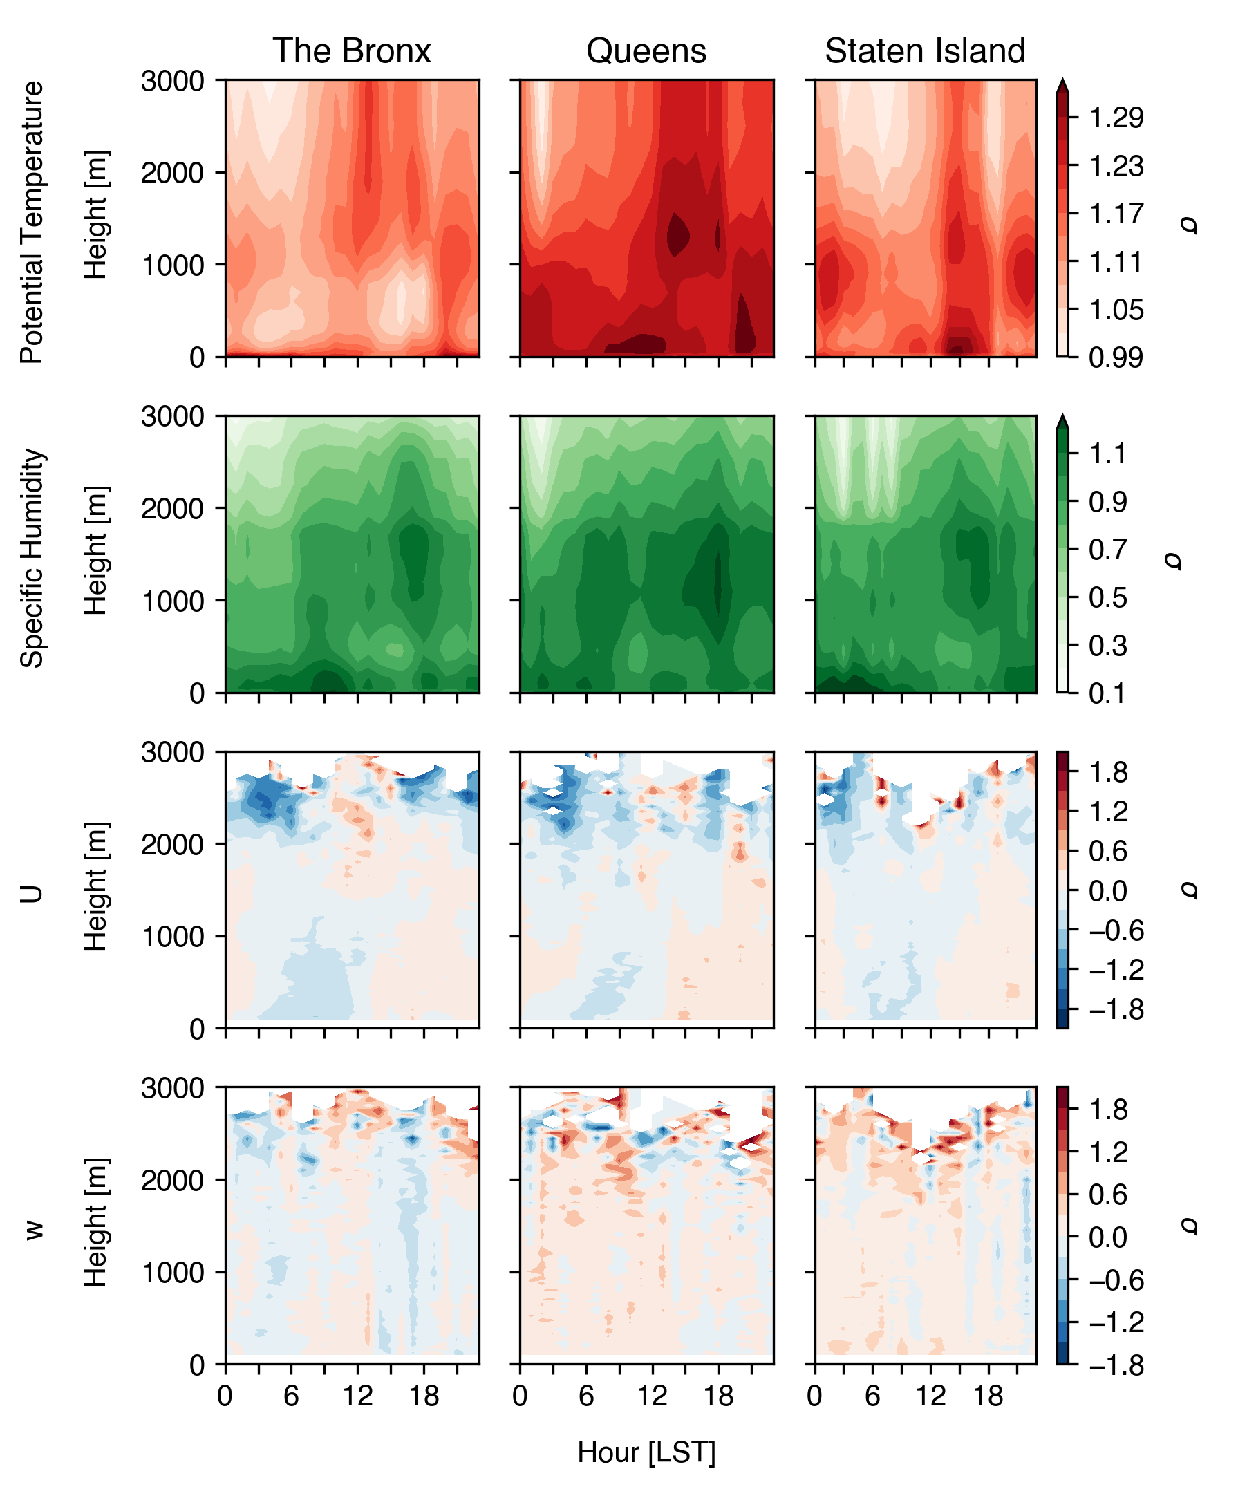
\includegraphics[width=0.75\textwidth]{Figures/heat_wave-normal-anomaly.png}
	\caption{Anomalies during extreme heat events relative to the climatology over the urban boundary layer.}
	\label{fig:extreme-heat-normal-comparison-contours}
\end{figure}

\begin{figure}[ht]
	\centering
	\includegraphics[width=0.75\textwidth]{Figures/heat_wave-normal-profiles-surface}
	\caption{Anomalies of temperature during extreme heat events relative to the climatology at the surface.}
	\label{fig:extreme-heat-normal-comparison-surface}
\end{figure}

\begin{figure}[ht]
	\centering
	\includegraphics[width=0.75\textwidth]{Figures/vertical_profiles-heat_wave-normal-theta.png}
	\caption{Vertical profiles of $\theta$ at the Bronx (a), Queens (b), and Staten Island (c) sites during normal days (blue) and extreme heat events (red).}
	\label{fig:vertical_profiles-heat_wave-normal-theta}
\end{figure}

\FloatBarrier

\subsection{Moisture}
On average, extreme heat events were found to increase the moisture at the surface, as indicated by the diurnal profiles of specific humidity ($q$) (see Figure \ref{fig:extreme-heat-normal-comparison-surface}). This is also consistent across all observed locations in New York City, with mean extreme heat event $q$ exceeding normal $q$ by approximately 1-$\sigma$ over the entire day. Although a distinct diurnal profile exists ($q$ decreases during daytime hours), the diurnal range is smaller in magnitude than temperature. It is also worth noting that the diurnal range is lower for Staten Island than for the Bronx or Queens, suggesting that degree of urbanization has a negative correlation with the diurnal range of $q$, due to sustained low-level moisture from local evapotranspiration from nearby vegetated areas. Similar to surface temperature, the variability of $q$ is significantly lower during heat events (average $ \sigma = \SI{2.14e-03}{\kilo\gram\per\kilo\gram} $) than during normal temperatures (average $ \sigma = \SI{3.18e-03}{\kilo\gram\per\kilo\gram} $). Queens shows exceptional variability in $q$, which may be attributed to the location of the observation site, which is adjacent to Flushing Meadows Corona Park (large open vegetated space), is surrounded by a medium-density urban area on all other sides, and is approximately \SI{4}{\kilo\meter} from Long Island Sound. 

In the boundary layer, the positive $q$ anomalies subside in magnitude between 300 and \SI{600}{\meter}, but increase significantly in the mixed layer, especially during the late morning and early afternoon for all sites. As shown in Figure \ref{fig:extreme-heat-normal-comparison-contours}, the largest anomalies occur between 10:00 and 16:00 LST throughout the mixed layer. With regards to spatial variation in $q$, Staten Island demonstrates a strong positive anomaly overnight through the early morning near the surface, indicating increased low-level moisture transport during extreme heat events, whereas the Bronx and Queens demonstrate a similar phenomenon with a lesser anomaly magnitude. All sites show significant positive $q$ anomalies throughout the day, with the strongest anomaly signal starting in the low-levels throughout the morning and transitioning to the mixed later by mid-afternoon. This trend suggests that the increase in nocturnal low-level moisture corresponds to increased UBL moisture content due to strong vertical mixing throughout the daytime.

This is supported by Figure \ref{fig:vertical_profiles-heat_wave-normal-q}, where vertical profiles of $q$ across all locations show markedly higher $q$ values at the surface during extreme heat events (approximately 1-$\sigma$), with $\frac{dq}{dz}$ values increasing throughout the morning in the mixed layer while low-level $q$ values decrease, indicating vertical transport of moisture and drier low-level conditions during peak insolation. The strong vertical mixing of $q$ can be observed at all sites, where late morning and early afternoon $\frac{dq}{dz}$ values are greater during extreme heat events than normal days. An example can be seen in the Bronx, where $\frac{dq}{dz} > 0$, indicating very efficient vertical moisture transport. 

In addition to environmental contributions to the positive $q$ anomalies during extreme heat events, it is known that anthropogenic contribution of water vapor increases during extreme heat periods. In New York City, most commercial buildings use chilled water coolers for air conditioning. For example, \citet{gutierrez2015} found significant contributions from the air conditioning system to atmospheric water vapor in the lower boundary layer. Similar findings were observed in Beijing \citep{yu2019} and Hong Kong \citep{wang2018}.

\begin{figure}[ht]
	\centering
	\includegraphics[width=0.75\textwidth]{Figures/vertical_profiles-heat_wave-normal-q.png}
	\caption{Vertical profiles of $q$ at the Bronx (a), Queens (b), and Staten Island (c) sites during normal days (blue) and extreme heat events (red).}
	\label{fig:vertical_profiles-heat_wave-normal-q}
\end{figure}

\FloatBarrier

\subsection{UBL dynamics}

\subsubsection{Horizontal winds}
Extreme heat events coincided with a modest reduction of horizontal wind speeds ($U$) in the UBL, as shown in Figure \ref{fig:extreme-heat-normal-comparison-surface}. More specifically, the magnitude of $U$ during extreme heat events is similar in magnitude to $U$ during normal days with the exception of early morning hours and at upper levels of the UBL. As shown in Figure \ref{fig:extreme-heat-normal-comparison-contours}, modest reductions in $U$ ($-1.2 \leq \sigma \leq -0.4$) during extreme heat events are present throughout the UBL from early to mid-morning, with little difference throughout the rest of the day ($-0.4 \leq \sigma \leq 0.4$). Larger deviations between $U$ values are present at the top of the UBL where synoptic conditions become dominant.

Vertical profiles of $U$ for normal and extreme heat events at specific hours provide a more detailed view of the differences in UBL structure. Across all sites, $U$ is similar throughout the UBL during afternoon, evening, and overnight hours. During early morning hours, however, extreme heat event $U$ values decrease by 25 to 50\% throughout the entire UBL (see Figure \ref{fig:vertical_profiles-heat_wave-normal-U}), although both event types present a classical logarithmic wind profile, with surface friction effects present through \SI{500}{\meter}. The reduction in $U$ during extreme heat events is likely due to the presence of an anticyclonic circulation that suppresses the nocturnal low-level jet over New York City \citep{chen1993}. Another phenomenon worth noting is the difference in $U$ profiles above \SI{2000}{\meter}; profiles of $U$ during extreme heat events are more consistent both vertically and spatially (between sites) than during normal days. This phenomenon demonstrates the effect of synoptic meteorological conditions on $U$, as the UBL typically remains below \SI{2500}{\meter}. During extreme heat events, anticyclonic conditions produce more consistent atmospheric conditions relative to normal days, resulting in less variability between heat events than during normal days.

Extreme heat events result in a southwesterly shift in $U$ throughout the UBL. This shift is present most evidently closer to the surface, as shown in Figures \ref{fig:wind_rose-bron}, \ref{fig:wind_rose-quee}, and \ref{fig:wind_rose-stat}, with winds at \SI{100}{\meter} coming primarily from the southwest quadrant. All sites also present secondary maxima with winds approaching from the south and southeast, which suggests effects from the Atlantic sea breeze (effects from the sea breeze will be further discussed in Section \ref{section:sea_breeze_effects}). At \SI{1000}{\meter}, the directionality of prevailing winds becomes more uniform between normal and extreme heat days, as winds primarily approach New York City from the west-southwest. The disparity in wind directions between 100 and \SI{1000}{\meter} suggests that localized wind fields play a more significant role in UBL dynamics at lower levels whereas synoptic-scale atmospheric conditions increasingly dominate with increasing height. Regardless, the uniformity of wind direction during extreme heat relative to normal days indicates that synoptic-scale effects can play a larger role at lower levels due to advection from the continent, especially with regards to thermal advection that leads to the transport of heated inland air masses over New York City \citep{jiang2019, ramamurthy2017b}.

\begin{figure}[ht]
	\centering
	\includegraphics[width=0.75\textwidth]{Figures/vertical_profiles-heat_wave-normal-U.png}
	\caption{Vertical profiles of $U$ at the Bronx (a), Queens (b), and Staten Island (c) sites during normal days (blue) and extreme heat events (red).}
	\label{fig:vertical_profiles-heat_wave-normal-U}
\end{figure}

% Standalone figure option
\begin{figure}[ht]
	\includegraphics[width=0.75\textwidth]{Figures/wind_rose-bron.png}
	\caption{Horizontal winds in the lower-level (100 m) and mid-level of the urban boundary layer over the Bronx.}
	\label{fig:wind_rose-bron}
\end{figure}
\begin{figure}[ht]
	\centering
	\includegraphics[width=0.75\textwidth]{Figures/wind_rose-quee.png}
	\caption{Horizontal winds in the lower-level (100 m) and mid-level of the urban boundary layer over Queens.}
	\label{fig:wind_rose-quee}
\end{figure}
\begin{figure}[ht]
	\centering
	\includegraphics[width=0.75\textwidth]{Figures/wind_rose-stat.png}
	\caption{Horizontal winds in the lower-level (100 m) and mid-level of the urban boundary layer over Staten Island.}
	\label{fig:wind_rose-stat}
\end{figure}

\FloatBarrier

\subsubsection{Vertical motion}
On average, extreme heat events do not appear to produce significant changes in vertical velocity ($w$) relative to normal days. Figure \ref{fig:extreme-heat-normal-comparison-surface} shows average diurnal profiles of $w$ at all locations at \SI{100}{\meter} above ground level, with similar mean values throughout the day between normal days and extreme heat events. During extreme heat events, the variability of $w$ is lesser in the early morning hours and greater in the evening, albeit featuring similar behavior to normal days. This phenomenon is also observed in vertical profiles of $w$ at all locations as shown in Figure \ref{fig:extreme-heat-normal-vertical_profiles-w}. At all locations, overnight and morning profiles of $w$ (0:00 and 6:00 LST) show significantly lower variability in $w$ throughout the UBL with similar magnitudes of mean $w$, although extreme heat days feature low variability in the UBL. Despite similar means and deviations in the early afternoon (12:00 LST), evening profiles (18:00 LST) show significantly higher variability in $w$ below \SI{500}{\meter} than in the mornings at the Queens and Staten Island sites, with the Bronx showing this occurrence extend through the UBL. The similarity in vertical profiles of $w$ may be a result of a balance between large-scale subsidence (due to the presence of high-pressure during extreme heat events) and the effects of increased surface forcings during extreme heat events relative to normal days \citep{dong2018, zhang2009}.

Additionally, updrafts appear to be lesser in magnitude relative to normal days, although upwards vertical motion persists later at all heights within the UBL. This suggests that vertical mixing is more sustained throughout the day during extreme heat events, although thermal plumes seem to be weaker relative to normal days. A case of this in shown at the Bronx site (see Figure \ref{fig:normal-extreme_heat-w-case_study}), where two days - 26 July 2019 (normal) and 29 July 2019 (extreme heat) - are shown with significantly different temporal profiles. On 26 July, the morning UBL is shallow and neutral through 10:00 LST, where mixing begins as evidenced by surface layer variability in $w$, which is followed by a sustained downdraft throughout the mixed layer. At approximately 12:00 LST, a strong plume extends throughout the UBL, initiating significant mixing from the surface throughout the mixed later. This is followed by modest downdrafts throughout the UBL in the afternoon, followed by relatively neutral conditions in the evening and early nighttime hours. In contrast, 29 July demonstrates similar UBL dynamics in the morning hours, followed by modest low-level mixing through the midday hours, with sustained upwards vertical motions through the afternoon and evening over the entire UBL. 

% Vertical quantity comparison timeseries, extreme heat versus normal
\begin{figure}[ht]
	\centering
	\includegraphics[width=0.75\textwidth]{Figures/vertical_profiles-heat_wave-normal-w.png}
	\caption{Vertical profiles of $w$ at the Bronx (a), Queens (b), and Staten Island (c) sites during normal days (blue) and extreme heat events (red).}
	\label{fig:extreme-heat-normal-vertical_profiles-w}
\end{figure}

% Case study of single day vertical velocity, comparison between normal and extreme heat day
\begin{figure}[ht]
	\centering
	\includegraphics[width=0.75\textwidth]{Figures/case_studies/normal-heat_wave-comparison_20190726_20190729-bron.png}
	\caption{Vertical velocity contours at the Bronx site on a normal (26 July 2019) and extreme heat (29 July 2019) day.}
	\label{fig:normal-extreme_heat-w-case_study}
\end{figure}

\FloatBarrier

%%%%% Discuss the observed sea breeze circulation
\section{Effects of the sea breeze circulation} \label{section:sea_breeze_effects} 
Sea breezes in New York City occur as a result of land-sea temperature gradients from two arms of the Atlantic Ocean; the New York Bight to the southeast and Long Island Sound to the northeast. Sea breezes from both bodies increase the complexity of UBL dynamics over New York City due to the coalescence of opposing fronts over the complex urban topography \citep{bornstein1981}. A typical sea breeze event in New York City is defined by calm ambient low-level winds ($\leq$ \SI{5}{\meter\per\second}), the formation of a large land-sea temperature gradient in the mid- to late morning, strong late-morning thermals that promote low-level convergence, and afternoon to early-evening onshore moisture transport and reduction in surface air temperatures (especially in areas closest to the shore) \citep{childs2005, frizzola1963, gedzelman2003}. 

Sea breeze events occurred on approximately 56\% of all days observed. The high frequency of occurrence is  attributable to low-level convergence due to the large land-sea temperature gradient that is common during warmer months \citep{childs2005, gedzelman2003, thompson2007}, as days were chosen exclusively between May and September. Maximum land-sea surface temperature differences during days with identifiable sea breeze events averaged at \SI{12}{\kelvin}, with a strong diurnal profile with the peak difference occurring around midday (see Figure \ref{fig:sea_breeze-lst_sst-diff}). The frequency of occurrence increases when observing days during extreme heat events, as the lack of a strong synoptic wind allows for the sea breeze circulation to become dominant in the metropolitan area \citep{miller2003}. 

% Sea breeze data
\begin{figure}[ht]
	\centering
	\includegraphics[width=0.75\textwidth]{Figures/sea_breeze-lst_sst-diff.png}
	\caption{Temperature difference between Queens and New York Bight.}
	\label{fig:sea_breeze-lst_sst-diff}
\end{figure}

\begin{figure}[ht]
	\centering
	\includegraphics[width=0.75\textwidth]{Figures/sea_breeze-normal-anomaly.png}
	\caption{Anomalies for normal days with a sea breeze relative to normal days without a sea breeze.}
	\label{fig:sea_breeze_normal-normal-anomaly}
\end{figure}

\begin{figure}[ht]
	\centering
	\includegraphics[width=0.75\textwidth]{Figures/sea_breeze_heat_wave-heat_wave_anomaly.png}
	\caption{Anomalies for heat wave days with a sea breeze relative to heat wave days without a sea breeze.}
	\label{fig:sea_breeze_heat_wave_anomaly}
\end{figure}

\FloatBarrier

\subsection{UBL structure during sea breeze events}
During normal days, observations show that the sea breeze reduces temperature and increases moisture content throughout the UBL after 12:00 LST. In Figure \ref{fig:sea_breeze_normal-normal-anomaly}, the standardized anomalies of $\theta$ between normal days with and without a sea breeze are shown, averaged over all days on an hourly basis. Overnight and in the early morning, positive anomalies of $\theta$ are present above the UBL ($\geq$ \SI{1}{\kilo\meter}) until mid-morning, with the Bronx having the most significant anomaly and Staten Island the least. This suggests a decreasing degree of anomalous $\theta$ with decreasing urbanization. This anomaly pattern coincides with a positive $q$ anomaly trend in both the spatiotemporal aspect (peak anomaly occurs above \SI{1}{\kilo\meter} before 8:00 LST) and the magnitude aspect (the Bronx has the most significant early morning anomaly, Staten Island has the least). Later in the day, all sites observe a negative $\theta$ anomaly throughout the UBL despite a negative $q$ anomaly, indicating that sea breeze events during normal days coincide with a cooler and drier daytime UBL before the onset of the sea breeze. Sea breeze effects become apparent during the mid-afternoon with the presence of a significant negative $\theta$ and positive $q$ anomaly in the lower UBL, with Staten Island experiencing effects first (approximately 16:00 LST) and the Bronx experiencing effects last (approximately 19:00 LST). This disparity in times appears to represent the passage of the southeasterly New York Bight, and to a lesser degree, the Long Island Sound sea breeze fronts through New York City, where the onset time correlates with the distance from the bodies of water \citep{bornstein1981}. It is worth noting that the $q$ anomaly is weakest in the Bronx, which suggests that the sea breeze front weakens as it travels inland over New York City.

During extreme heat events, observations show that the sea breeze plays a moderating role on surface conditions by reducing low-level temperatures and increasing low-level moisture content, similar to phenomena observed during normal days. In Figure \ref{fig:sea_breeze_heat_wave_anomaly}, the standardized anomalies of $\theta$ between extreme heat days with and without a sea breeze are shown, averaged over all days. All sites shown that extreme heat days with a sea breeze possess slightly higher values of $\theta$ in the mid-morning, with significant low-level reduction in $\theta$ in the afternoon and evening. On average, the onset of the low-level cooling occurs in Staten Island first at approximately 12:00 LST, with Queens following at approximately 14:00 LST, and the Bronx at about 18:00 LST. It is worth noting that the negative $\theta$ anomalies are stronger in more urbanized areas, as shown by the Bronx and Queens sites. A similar phenomenon is observed by the transport of $q$ as shown in Figure \ref{fig:sea_breeze_heat_wave_anomaly}, with drier conditions throughout the UBL before 12:00 LST and increasing low-level moisture as the day progresses. With regards to onset, $q$ follows a similar pattern to $\theta$ in that the onset time is dependent from distance to the shore. These anomalies present most significantly in the lowest \SI{1000}{\meter} of the UBL after 12:00 LST, which aligns with sea breeze circulation characteristics observed in \citet{frizzola1963}.

\subsection{UBL dynamics during sea breeze events}
Days with identifiable sea breeze events had lower $U$ throughout the majority of the UBL, with the most significant decreases during the nighttime, potentially due to the lessening of onshore flow due to the reduction of the land-sea temperature gradient \citep{pullen2007}, as shown in Figure \ref{fig:sea_breeze-lst_sst-diff}. Vertical motions, however, increased significantly in the Bronx and Queens during the late morning and early afternoon, as shown in Figure \ref{fig:sea_breeze_heat_wave_anomaly}. These anomalies indicate the increased presence of updrafts in urbanized areas which contribute to low-level convergence and the initiation of a localized sea breeze circulation, promoting onshore flow in the afternoon and evening.

During extreme heat days with identified sea breeze circulations, easterly winds increase in frequency in the lower levels of the UBL, as shown in Figure \ref{fig:wind_direction-heat_wave-sea_breeze-histogram}. These winds are the result of onshore flow from the New York Bight (southeasterly) and Long Island Sound (northeasterly). 

During extreme heat days with sea breeze circulations, southeasterly winds increased in frequency compared to all other directions at all locations. The occurrence frequency of southeasterly winds is correlated with the distance between the observation site and the largest body of water in proximity of the metropolitan area (Atlantic Ocean), as Staten Island reported 92.1\% of all winds at \SI{100}{\meter} as southeasterly between 12:00 and 20:00 LST (distance of \SI{6.50}{\kilo\meter} from Lower New York Bay), whereas Queens reported 67.4\% (distance of \SI{16.5}{\kilo\meter}) and Bronx reported 55.6\% (distance of \SI{32.9}{\kilo\meter}) during the same time interval. The disparity in southeasterly winds further demonstrates the spatial extent and progression of the sea breeze front.

For sites near Long Island Sound (the Bronx and Queens), northeasterly winds increased in frequency as well, though not to the same magnitude as southeasterly winds. This disparity in magnitude suggests that the Long Island Sound sea breeze front is weaker than the New York Bight sea breeze front, which aligns with previous studies of sea breeze fronts over New York City \citep{frizzola1963, meir2013}. Northeasterly winds increased in frequency during extreme heat days with sea breeze circulations, with a notable increase in the early morning hours (a likely result of nocturnal low-level motion) and in the evening hours (signal of a Long Island Sound sea breeze). This phenomenon is also apparent in Queens and Staten Island, albeit to a lesser frequency. 

% Histograms cataloguing frequency of wind directions at 100 m between heat wave days without and with a sea breeze.
\begin{figure}[ht]
	\centering
	\includegraphics[width=0.75\textwidth]{Figures/histogram-wind_direction-sea_breeze-100m.png}
	\caption{Occurrence frequency of wind directions during (a) extreme heat days without a detected sea breeze and (b) heat wave days with a detected sea breeze, at \SI{100}{\meter} at all sites.}
	\label{fig:wind_direction-heat_wave-sea_breeze-histogram}
\end{figure}

\FloatBarrier

\section{Discussion and conclusions} \label{section:discussion_conclusion}

% Supporting evidence
Several phenomena observed in this study have been noted in the literature. With regards to heat-related phenomena, the 'heat dome' effect observed through comprehensive multi-city airborne observations in \citet{zhang2020} was observed herein, with a notable increase in temperatures ($\sigma \geq 0.99$) throughout the UBL during extreme heat events. Specifically, the peak temperature anomalies during extreme heat events occurred during the early morning and early afternoon in the surface layer, with secondary maxima in the mixed layer at approximately \SI{1500}{\meter}. The climatology of mixed layer properties provided in this study aligns with findings herein using different observational methods, although on single-city scale, which is beneficial towards understanding the effects of extreme heat within cities and improving our understanding of the relationship between the surface and mixed layers. It is worth noting that this behavior is similar to modeled conditions presented by \citet{ortiz2018} from a series of factor-separation studies using the Weather Research and Forecasting (WRF) model to understand the effects of urbanization on meteorological conditions in New York City. The results showed that surface factors from urban land cover types presented substantial increases to the surface and mixed layer temperatures (6 to \SI{8}{\kelvin} throughout the day). Moreover, simulations showed especially robust early morning (6:00 LST) mixed layer increases in $\theta$ during extreme heat events, which aligns with composite observations shown herein, despite the studies only ranging over a 5-day period for a specific extreme heat event.

With regards to moisture-related phenomena, various studies have shown that there is increased UBL moisture content during extreme heat events \citep{kunkel1996, pyrgou2020, zhang2020}. In particular, the positive anomalies of $q$ are strongest in the surface layer during the morning, which aligns with findings from the Midwestern United States \citep{kunkel1996} and various regions of differing climates \citep{zhang2020}. However, to the authors' knowledge, very few studies have catalogued long-term observations of the vertical structure of moisture in the UBL during extreme heat events. \citet{zhang2020} presented comparisons of the average diurnal vertical structure of $q$ in humid regions (Louisville, Houston, and Philadelphia) and an inland city in a dry inland region (Denver) and showed the differences in the UBL $q$. Louisville and Philadelphia experienced increases in $q$ throughout the UBL, whereas Houston and Denver experienced decreases in low-level $q$, despite Houston being a coastal city in a humid region. This phenomenon was attributed to synoptic-scale moisture transport, where moist air masses from surrounding humid areas paired with local evapotranspiration to increase $q$ in Louisville and Philadelphia, but drier air masses from the Mountain West resulted in lower $q$ values during extreme heat events. The effects of extreme heat on $q$ in New York City resemble those of the cities in humid regions, where humid continental air masses paired with evapotranspiration from vegetated areas surrounding the area to increase $q$ substantially ($0.1 \leq \sigma \leq 1.2$). The influence of localized UBL dynamics (i.e., sea breeze) further increased low-level $q$ as a result of onshore moisture transport, especially during nighttime hours. 

On a larger scale, differences in UBL dynamics have been shown to play a major factor in UBL properties between normal and extreme heat days. As shown herein, a southwesterly shift in winds throughout the UBL coincided with extreme heat events, further highlighting the role of synoptic conditions on the UBL during extreme heat. The increase in temperatures due to this shift in winds has been reported in multiple studies \citep{heaviside2015, jiang2019, ramamurthy2017b}, where the shift in wind direction results in advection of hot air from continental land masses or the advection of heat from nearby urban areas. In the case of New York City, a southwesterly shift in winds places New York City downwind of the continental United States and the north-central New Jersey urban conurbation, both of which may contribute to a hotter UBL during extreme heat events. Moreover, the effect of sea breezes from multiple fronts around New York City creates a complex flow pattern that increases spatial variability in the local meteorology, which has been shown to reduce temperature throughout the UBL \citep{han2022, hirsch2021, lee2021}, albeit contributing to higher moisture content which affects the nocturnal and successive morning UBL structure. 

% Errors and future work
Despite the extensive results provided herein, additional work is required to better improve our understanding of neighborhood-scale spatial qualities of the boundary layer throughout urban areas, especially in those with complex topography and land cover attributes, such as a coastal city. Despite observation sites in 3 of the 5 boroughs, New York City also features a highly variable array of land cover types and features that are not represented in this study. For example, targeting areas in the densest parts of the city (e.g., Midtown Manattan) or furthest from the coast (e.g., central Brooklyn) would be ideal for observing UBL properties in areas of the city most likely to have peak surface temperatures. The variability of building heights throughout New York City, especially in Manhattan, further complicates UBL dynamics and downwind transport \citep{hanna2006, hanna2007}. Moreover, the distance between sites is on the order of the size of a borough, rendering each station unable to be fully representative of neighborhood-scale processes. A potential solution includes a more extensive network of weather and profiling stations (the Oklahoma City Micronet and its usage as described by \citet{basara2010} is a useful example) that allows for more land cover types to be represented.

% Answer the scientific questions posed in the introduction
Based on the observations and their derived quantities, insight was provided into the questions posed in Section \ref{section:introduction};

\begin{enumerate}
	\item Regarding UBL structure, the UBL shows increased temperatures and moisture content throughout its entirety during extreme heat events. Specifically, the surface and lower mixed layer show the most significant increases in temperature and moisture throughout the diurnal cycle. Moreover, the afternoon mixed layer presents a secondary maxima in temperature and moisture increases, suggesting more sustained vertical mixing during extreme heat events. Regarding UBL dynamics, horizontal wind speeds are slightly lower on average during extreme heat events, with the most notable reductions present in the early morning hours and at the UBL height. Additionally, the directionality of horizontal winds becomes predominantly southwesterly and uniform across the UBL during extreme heat events, suggesting increased low-level advection from the continental United States. Differences in vertical motions between normal days and days with extreme heat are not significant when averaged, although extreme heat events were found to correlate with weaker updrafts despite sustaining prolonged positive $w$ values through the evening hours. Extreme heat days were also found to be less variable in terms of UBL structure and dynamics relative to normal days.
	\item Locally, the transport of scalars appears to increase in the vertical direction during extreme heat events in the UBL, although decreased low-level horizontal winds suppresses strong scalar transport zonally and meridionally, especially during morning hours. Despite similar vertical rates of change of scalar quantities between normal days and days with extreme heat, the increase in low-level temperature and moisture content results in significantly higher mixed layer temperature and specific humidity values during extreme heat days. Moreover, extreme heat days appear to promote onshore low-level moisture transport, especially in areas immediately adjacent to the coast. This phenomenon coincides with an increased sea breeze event frequency during extreme heat events. On a larger scale, the vertical uniformity in wind direction throughout the UBL during extreme heat events promotes the advection of scalars southwest of New York City. 
	\item The sea breeze reduces temperatures throughout the UBL after the onset of the sea breeze, which typically occurs in the mid-afternoon in immediate coastal areas and in the evening for areas further inland. The sea breeze also results in nocturnal low-level onshore moisture transport. It is worth noting that during normal days, there was no significant difference in vertical velocities during days with a sea breeze relative to days without a sea breeze, despite a significant reduction in horizontal winds. However, extreme heat days, significantly higher $w$ values occurred through the surface and lower mixed layer during the late morning periods at the Bronx and Queens sites.
	
\end{enumerate}

\section*{Appendix} \label{section:appendix}

\subsection*{Atmospheric pressure}

Atmospheric pressure, $p$, was derived using Equation \ref{eqn:pressure} from observed surface pressure ($p_0$), observed surface temperature ($T_0$), height above the surface ($p$), and the gas constant for dry air ($R$) following the definition provided in \citet{wallace2006}. Note that the virtual temperature correction is neglected in this derivation.

\begin{equation*}\label{eqn:pressure}
	p = p_0 \exp{\frac{-g z}{R T_0}}
\end{equation*}

\subsection*{Potential temperature}

Potential temperature ($\theta$) was derived using Equation \ref{eqn:potential_temperature}, using observed surface temperature ($T_0$), observed surface pressure ($p_0$), height above the surface ($z$), and the gas constant for dry air ($R$), following the definition provided in \citet{wallace2006}.

\begin{equation*}\label{eqn:potential_temperature}
	\theta = T \left(\frac{p_0}{p} \right)^{\frac{R}{c_p}}
\end{equation*}

\subsection*{Specific humidity}

Specific humidity ($q$) was derived using Equation \ref{eqn:specific_humidity} as a function of the mixing ratio ($w$), which in turn is a function of the density of water vapor (also known as \textit{vapor density}) ($\rho_v'$), air temperature ($T$), and the gas constant for water vapor ($R_v$), following the definitions provided in \citet{wallace2006}. 

\begin{equation*}\label{eqn:specific_humidity}
	q = \frac{w}{1+w} = \frac{\frac{\varepsilon \rho_v' R_v T}{p - \rho_v' R_v T}}{1+\frac{\varepsilon \rho_v' R_v T}{p - \rho_v' R_v T}} 
\end{equation*}

% Table displaying symbols used in the 
\captionof{table}{Symbols and abbreviations used in the chapter.}
\label{tab:symbols}
\begin{center}
	\renewcommand{\arraystretch}{1}%
	\begin{tabularx}{0.75\textwidth}{l X}
 		\hline
 		Symbol/Abbreviation & Definition \\
 		\hline
 		$\sigma$ & Standard deviation \\
 		$\theta$ & Potential temperature \\
 		$q$ & Specific humidity \\
 		$U$ & Horizontal wind speed \\
 		$w$ & Vertical velocity \\
 		UBL & Urban boundary layer \\
 		\hline
	\end{tabularx}
\end{center}
\cleardoublepage

% -------------------------------------
% CHAPTER 5: CONCLUSIONS
% -------------------------------------
\chapter{Conclusions and Future Work}
\label{chapter:Conclusions}
\thispagestyle{myheadings}

\graphicspath{{4_Conclusion/Figures/}}

This thesis provides insights into the capabilities of remote sensing for improving observations such that our understanding of the UBL can be improved. In this chapter, results from the work done to establish these capabilities and the associated findings are summarized in Section \ref{section:summary}. The limitations of the methods used will also be discussed in Section \ref{section:limitations}, as there are many improvements that can be made upon the methods used herein. In addition to the limitations and possible improvements, the potential directions the work performed could be taken in to build upon this topic will be discussed in \ref{section:future_work}.

\section{Summary}\label{section:summary}

This thesis contributes novel findings regarding UBL structure, dynamics, and energy exchange with a focus on using remote sensing methods to drive analysis of the UBL. This begins with Chapter \ref{chapter:goes}, where a lightweight algorithm is presented that uses GOES-R satellite data and a \SI{2}{\meter} air temperature machine learning method to estimate $Q_H$ in urban areas. This work is relevant to urban meteorology and remote sensing of surface processes, as it presents a new and portable method to leverage operational satellite data for real-time estimation of surface fluxes. The satellite-derived estimates of $Q_H$ were validated by comparison to several flux towers in New York City, with a resulting $R^2$ value of 0.70 and an MBE of \SI{16.58}{\watt\per\meter\squared}. This work resulted in a peer-reviewed journal publication \citep{rios2022novel} and has shown to outperform a dedicated urban numerical weather prediction model with regards to the estimation of $Q_H$. Additionally, this work demonstrated the spatial and temporal variability of $Q_H$ within New York City. In terms of spatial variability, higher values of $Q_H$ were presented in highly-urbanized neighborhoods with minimal vegetation, indicating that $Q_H$ is responsible for the majority of the urban surface energy balance and that higher values of $Q_S$ are present in these areas. In terms of temporal variability, a seasonal cycle of $Q_H$ was apparent with spring and summer months exhibiting the strongest surface fluxes. 

To supplement the usage of satellite-derived data to improve our understanding of UBL processes, the work performed in Chapter \ref{chapter:climatology} used ground-based remote sensing methods to vertically-profile the UBL to analyze UBL structure and dynamics with an emphasis on UBL behavior during extreme heat events. In this chapter, lidar and microwave radiometers, situated in 4 boroughs and operating for 3 years continuously, are used to provide long-term observations of the UBL over New York City. The number of stations, coupled with a maximum vertical resolution of \SI{100}{\meter}, allows for a comprehensive spatial analysis of the UBL in a large and diverse coastal urban area. Particular focus was given to extreme heat events, which present a significant natural hazard for New York City. Findings from observations and the successive analysis indicate that extreme heat events present a site-averaged \SI{2}{\meter} air temperature increase of \SI{7}{K} for daily high temperatures, with a 39.4\% increase in specific humidity and a southwesterly shift in winds throughout the entirety of the UBL. Moreover, extreme heat events present a statistically-significant increase to temperature and moisture throughout the vertical extent of the UBL. It was also observed that sea breezes from the Atlantic Ocean and Long Island Sound contributed to reduced afternoon and evening temperatures and were critical for onshore moisture transport during nighttime hours, although these effects were directly proportional to the distance of the observation site from these bodies of water. Findings from this work have resulted in a submission to a peer-reviewed journal and are aimed to improve the understanding of how extreme heat events affect conditions both at the surface, but also throughout the UBL, as a proper understanding of the UBL is critical for improving modeling and forecasting methods.

\section{Limitations}\label{section:limitations}

Various limitations affected the work performed herein. Methods to address these limitations are discussed in Section \ref{section:future_work}. 

With regards to the satellite-driven algorithm for $Q_H$ estimation presented in Chapter \ref{chapter:goes}, the heterogeneity of urban surfaces is a parameter that presents shortcomings to propertly estimating surface fluxes throughout an area with land cover surface properties as complex and variable as in New York City. The usage of satellite data with \SI{2}{\kilo\meter} resolution, while more than sufficient for many application, is limited for areas with such granular surface properties. The inability to capture surface properties at lower resolutions using this satellite dataset was identified as a key contributor to estimation errors during the validation process for this product. Additionally, the complex flow structure presented by the urban canopy in New York City creates a highly heterogeneous flow environment that can lead to intra-neighborhood variability in surface fluxes at a resolution that is not captured by the model. 

With regards to the observations and analysis using ground-based remote sensing methods presented in Chapter \ref{chapter:climatology}, a key shortcoming is the fact that each observational site performed is a single point, geographically speaking. In an environment as complex as New York City, a point is insufficient to capture the microscale turbulence that occurs as a function of differential building heights and surface cover types that can change within a matter of meters. Although the usage of sites from several boroughs attempts to provide some sort of spatial variability, the results presented may vary to some degree from one block to the next. This is especially true for observations made within the roughness sublayer, as mixing is driven by turbulent processes arising from surface properties.

\section{Future Work}\label{section:future_work}

The fields of urban meteorology and boundary layer research are constantly evolving and will be increasing in societal relevance due to the increasing degree of urbanization globally and the effects of climate change. Given this, the work presented here can be expanded upon and be a stepping stone to much greater findings with social and technical impacts.

The work presented in Chapter \ref{chapter:goes} can readily be applied to derive surface latent heat fluxes ($Q_L$) using satellite data. The critical step to adapt the algorithm for $Q_H$ towards estimating $Q_L$ involves the incorporation of a method to estimate evaporation and transporation in urban areas. These factors will be functions of vegetation, soil moisture, and bodies of water within urban areas that contribute to vertical moisture transport and horizontal advection. Additionally, the application of both of these methods could prove useful for validation of numerical weather prediction models, as the algorithm adds a spatial extent that builds upon the point-based observation data provided by flux towers that is currently used for validation. This validation method may be able to assist research into improvements for these models, especially in urban areas, where numerical models may fail to capture local-scale atmospheric phenomena. Upon completion of the algorithm for $Q_L$, a complete satellite-based notable step forward in identifying the individual components of the surface energy budget. This has crucial implications for fields such as urban planning and public health, as mitigation and placement strategies can be informed by understanding the factors that contribute to surface energy budget components and their relationships to heat and human comfort. 

The work presented in Chapter \ref{chapter:climatology} is currently being expanded upon to focus on UBL dynamics. The focus on UBL dynamics is important because of the work needed to better understand turbulence throughout the UBL. A specific emphasis is being placed on the relationship between the surface and mixed layers, as their interface (the roughness sublayer) has been found to be a layer within which MOST fails to capture turbulent processes. The analysis of turbulence in the UBL is being performed with several high-resolution lidars to capture a wide range of turbulent processes, with the aim of using methods such as spectral analysis and statistical filters to identify turbulent eddies, mixing timescales, and the differences between turbulent properties at different levels in the UBL. 

\cleardoublepage

%==========================================================================%
% Bibliography
\newpage

% each subdirectory can have its own BiBTeX file
% \bibliography{thesis}
\printbibliography
\cleardoublepage

%==========================================================================%
\end{document}
